
\documentclass{MScthesisITEM}

% this package is just to generate text for demo-purposes

\usepackage{mathtools}
\usepackage{amsmath}
\usepackage{listings}
\usepackage{framed}
\usepackage{underscore}
\usepackage{parskip}
%\usepackage[toc][acronym]{glossary}
%\usepackage[nonumberlist]{glossaries} 

\usepackage[nonumberlist,acronym,xindy,toc]{glossaries} % nomain, if you define glossaries in a file, and you use \include{INP-00-glossary}
%\makeglossaries
\usepackage[xindy]{imakeidx}
\makeindex

\title{Utilizing Mesh Potatoes in Emergency \\ Situations} % The title of your assignement; NB use \newlinetitle to start a newline
\author{Esther Bloemendaal \& Ida Malene Hassel Øveråsen}
\professor{Norvald Stol, ITEM} % Affiliation = ITEM for instance
\supervisor{Sjur Eivind Usken, Aarbakke Innovation AS}

%% Uncomment the following in case you want subfigures; note that there will be a warning for the caption package
\let\subcaption\undefined
\let\subfloat\undefined
\usepackage[bf]{caption}
\usepackage{subcaption}


\DeclareGraphicsExtensions{.pdf,.jpg}
\graphicspath{{./figs/}}

\loadglsentries{glossary.tex}
\makeglossaries



\begin{document}
\selectlanguage{english}
\pagenumbering{roman}
\pagestyle{plain}

%% Only for the project

\titleITEM

%% Only for the master's thesis; for the project report the description is taken from It's Learning and added by the department
% \selectlanguage{english} % Change to 'norsk' if you are writing in Norwegian
% \begin{titlingpage}

\noindent
\begin{tabular}{@{}p{4cm}l}
\textbf{Title:} 	& \thetitle \\
\textbf{Student:}	& \theauthor \\
\end{tabular}

\vspace{4ex}
\noindent\textbf{Problem description: }
Village Telco is an organization that aims to provide the solution for local communities can deploy data and voice services where no other companies can, or are willing to do so. Village Telco provides a “plug-and-play” solution with low cost voice and data service. While designed for the developing world, Village Telco’s solution can be applied anywhere where people wish to take control of their own telephone infrastructure.

This solution is delivered using an inexpensive fixed mesh WiFi delivery system called the Mesh Potato. The MeshPotato unit is based on the open-source operating system, OpenWRT. Open Source telephony software combined with the latest wireless networking technology creates the potential for people to operate their own community phone systems. Mesh Potato networks have no dependence on existing telecom infrastructure, and can relatively easily be deployed anywhere in the world. It can either be deployed as a stand-alone solution or as an extension to existing technologies. Village Telco’s solution has been deployed in several countries around the world: from East-Timor and Nepal in Asia to several African and South American countries. The installed bases vary from 10 to several hundreds of Mesh Potatoes. 

An area that has not been fully explored is the use of Mesh Potatoes in emergency situations, like natural disasters, post-conflict situations, etc. Another area to be considered is the use of Mesh Potatoes in refugee camps, where many people quickly gather in a new location. In both situations, the need for communication is essential. Key factors of usage are quick roll-out and usability. Easy to use communication is extremely important in crisis situations, both communication within the camp and outgoing communication with the rest of the world. It is important that all affected have easy access to helpful information, as this could mean the difference between life and death in some situations. In refugee camps with thousands of people, registering and reuniting people can be a difficult task to solve. Communication technology, like the Mesh Potato, could be revolutionary in situations like these. 

We will look into how communication is handled by Norwegian emergency relief organizations today, what tools they are using, and if their way of communication could improve with the Mesh Potato. In addition to this, we will look into other existing tools, and explore the possibilities to combine them with the Mesh Potato for a better product.

\vspace{2ex}

\noindent \Blindtext[2][1]
\vspace{6ex}

\noindent
\begin{tabular}{@{}p{4cm}l}
\textbf{Responsible professor:} 	& \theprofessor \\
\textbf{Supervisor:}			& \thesupervisor \\
\end{tabular}

\end{titlingpage}
% \cleardoublepage

%% There must be an abstract in English, even though the main text is in Norwegian
\selectlanguage{english}
\renewcommand{\abstractname}{Abstract}
\begin{abstract}

The Village Telco organization aims to provide affordable communication by means of data and voice services where no other companies are able or willing to do so. Village Telco provides a “plug-and-play” solution with low cost voice and data service. This solution is delivered using an inexpensive fixed mesh WiFi delivery system called Mesh Potato. Village Telco’s solution can be applied anywhere in the world where people wish to take control of their own communications infrastructure. Mesh Potato networks can be deployed either as a stand-alone solution or as an extension to existing technologies. Village Telco’s solution has been deployed in several countries around the world. The installed communities vary from ten, to several hundreds of Mesh Potatoes. 

We directed our studies toward the use of Mesh Potatoes in mobile situations. We have looked at different scenarios covering everything from emergency situations and natural disasters, to festivals and temporary refugee camps. Keith Williamson, a Village Telco volunteer, has created a "go box" using the first generation of the Mesh Potato. We wanted to take his solution further and developed a mobile and stand-alone kit that could be used in all the different scenarios mentioned. The prototype we have developed is slightly different from the "go box". We have used the second generation Mesh Potato and the box includes everything necessary for a quick roll-out; solar panel, battery, different cables and easy to use manuals for configuration. 

We established that many of the descriptions found on the Village Telco wiki were not clear and difficult to use. Hence a big part of our work consisted in simplifying these descriptions. We created manuals for connecting the Mesh Potato to different uplinks in order to provide Internet access to the network. Four test persons, both with and without technical knowledge, tested the manuals. The test process gave us valuable feedback, which led to improvements in the manuals. We have looked at the process of roll-out, and stated possible simplifications and improvements in order to make the roll-out as quick as possible. Hence we have named our solution the \gls{quick} box.

We believe that our work and theoretical research has contributed to and enriched the Village Telco community. Our prototype can be further developed and introduced to relief organizations as well as to others who express an interest in a mobile communications kit. 


\end{abstract}

\cleardoublepage

%% Only for the master's thesis; if the main text is in English and you can write Norwegian, there must be an abstract in Norwegian as well.A
%\selectlanguage{norsk}
%\renewcommand{\abstractname}{Abstract}
\begin{abstract}


* Hvorfor vi gjør det som vi gjør, hva er bakgrunnen

* Hva har vi gjort

* hvordan har vi gjort det

* hva fant vi ut

* hva resulterer det i hva konkluderer vi med?



Village Telco is an organization that aims to provide affordable communication in forms of data and voice services where no other companies can, or are willing to do so. Village Telco provides a “plug-and-play” solution with low cost voice and data service. While designed for the developing world, Village Telco’s solution can be applied anywhere people wish to take control of their own communication infrastructure.

This solution is delivered using an inexpensive fixed mesh WiFi delivery system called the Mesh Potato. The Mesh Potato unit is based on the open-source operating system, OpenWRT. Open Source telephony software combined with the latest wireless networking technology creates the potential for people to operate their own community phone systems. Mesh Potato networks have no dependence on existing telecom infrastructure, and can relatively easily be deployed anywhere in the world. It can either be deployed as a stand-alone solution or as an extension to existing technologies. Village Telco’s solution has been deployed in several countries around the world: from East-Timor and Nepal in Asia to several African and South America countries. The installed bases vary from 10 to several hundreds of Mesh Potatoes. 

We have directed our studies toward the use of Mesh Potatoes in mobile situations. We started by looking into different scenarios consisting of everything from emergency situations and natural disasters, to festivals and temporary refugee camps. After being in contact with different relief organization we got a clear impression that communication under and after a disaster situation is a difficult task. Keith Williamson, a Village Telco volunteer, has created a "go box" using the first generation of the Mesh Potato. We wanted to take his solution further and develop a mobile and stand-alone kit that could be used in all the different scenarios that we have taken into consideration. The prototype we developed differs from the one already made. We have used the second generation Mesh Potato and the box includes everything necessary, solar panel, battery, different cables and easy to use manuals for configuration. 

In the process of creating this kit we had to set up the network in order to conduct testing, both of the network and the configurations. We found that many of the descriptions found on the Village Telco wiki were little explanatory and difficult to use. Therefore a big part of our work has been to simplify these descriptions, and make them easy that little or non-technical people can use and understand them. We have looked at simplifications as well as processes in order to make the roll-out as quick as possible. Hence we have named our solution the \gls{quick} box.

* Fylle ut mer her etter at vi har skrevet konklusjonen

We believe that our work and theoretical research has contributed and richened Village Telco. And eventually save lives. 






\end{abstract}
%\cleardoublepage

\selectlanguage{english}% Change to 'norsk' if you are writing in Norwegian

\renewcommand{\abstractname}{Preface}
\begin{abstract}

This study was performed as a master's thesis on behalf of the \gls{item} at the \gls{ntnu}, in cooperation with Village Telco. This report is the final result of this master's thesis and is worth 30 ECTS points. The study was conducted between January and June 2014. The project description was outlined in cooperation with our project supervisor Sjur Usken from Aarbakke Innovation AS.

We would like to thank Sjur Eivind Usken who has guided us throughout our project, and contributed with helpful ideas, feedback and support. We would also like to thank our project professor Norvald Stol for his helpful feedback and support. We thank the Village Telco community, especially Steve Song and Keith Williamson, for taking the time to answer our questions and for helping us along the way. Also a thanks to Marte Berg Innset for the collaboration on the background chapter. Finally, we would like to thank everyone who helped us test the prototype of the QUICK box. \\

\vspace*{2\baselineskip}
\paragraph{}
Trondheim, June 11, 2014
\vspace*{1.5\baselineskip}
\paragraph{}
Esther Bloemendaal
\paragraph{}
Ida Malene Hassel Øveråsen


\end{abstract}
\cleardoublepage

% similarly you may add a separate acknowledgments page

\tableofcontents*
\cleardoublepage

%% include if relevant
\listoffigures
\cleardoublepage

%% include if relevant
\listoftables
\cleardoublepage

%% include if relevant
%\listofalgorithms
%\addcontentsline{toc}{chapter}{List of Algorithms}
%\cleardoublepage

%% include if relevant
\glsaddall[]
%\printglossaries%[title=List of Symbols, style=long]
%\cleardoublepage


%% include if relevant
\printglossary[title=List of Acronyms,type=\acronymtype] % prints just the list of acronyms
\cleardoublepage

\pagenumbering{arabic}
\pagestyle{ruled}

\chapter{Introduction}
\label{chp:introduction} 
%% include here the other chapters
\chapter{Background}
\label{chp:background} 

\section{Village Telco}
%How did it all start?

\section{Mesh Potato}
%Generelt om MP

% hvordan MPen fikk navnet. 


%MP01
<<<<<<< HEAD
The whole concept around the Mesh Potato was developed in June 2008 during a workshop with the Village Telco team. The aim was to develop a business model as well as a prototype for a Villa Telco. Initially the idea was to use low cost VoIP headsets. At the time this was the most viable and convenient way to deliver telephone services to the customers. With a VoIP telephone service the nodes can not be more that 100 meters away from each other, requiring more nodes to be able to cover the desirable area. Which again drastically increases the start-up costs for a village. In order to keep the cost down, it was also important to keep the number of access points down. A mesh network have a larger range, and one suggestion was to use a small mesh device like a Open Mesh AP and connect a SIP phone to it. This solution would solve a lot of the problems regarding range, antenna and number of access points, but the idea was still an expensive option. During the debating, Rael Lissoos took a Analouge Telephone Adapter (ATA) and an Open Mesh AP, held them together and said that we need these two devices in one. This point was the birth of the Mesh Potato. The name comes from combining the words mesh, POTS (Plain Old Telephone) and ATA. Patata is the Spanish word for potato, and hence the name Mesh Potato. A mesh enabled WiFi device with the possibility to connect any inexpensive regular phone and IP device. \cite{MPorigin}
=======
The whole concept around the Mesh Potato was developed in June 2008 during a workshop with the Village Telco team. The aim was to develop a business model as well as a prototype for a Village Telco. Initially the idea was to use low cost VoIP headsets since it was the most viable and convenient way to deliver telephone services to the customers. With a VoIP telephone service the nodes can not be more than 100 meters away from each other requiring more nodes to be able to cover the desirable area. Which again drastically increased the start-up costs for a village. In order to keep the cost down, it is also important to keep the number of access points down. A mesh network have a larger range, and one suggestion was to use a small mesh device like a Open Mesh AP and connect a SIP phone to it. This solution would solve a lot of the problems regarding range, antenna and number of access points, but the idea was still an expensive option. During the debating, Rael Lissoos took a Analouge Telephone Adapter (ATA) and an Open Mesh AP, held them together and said that we need these two devices in one. This point was the birth of the Mesh Potato. The name comes from combining the words mesh, POTS (Plain Old Telephone) and ATA. "Patata" is the Spanish word for potato, and hence the name Mesh Potato. A mesh enabled WiFi device with the possibility to connect any inexpensive regular phone and IP device. \cite{MPorigin}
>>>>>>> 48118eeb54d92f9fb9eb7897a927417878f85a17

\begin{figure}[h!]
  \centering
      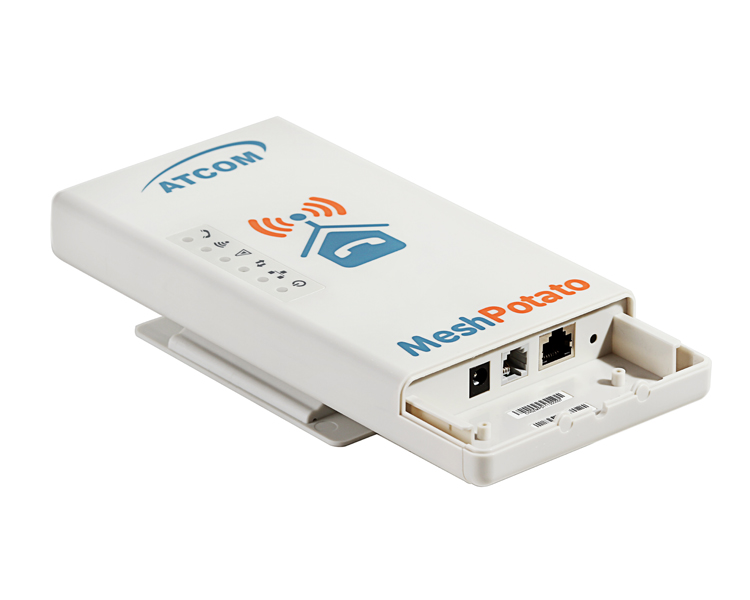
\includegraphics[width=0.5\textwidth]{MP01}
  \caption [The Mesh Potato]{\textbf{The fist generation Mesh Potato, MP01}}
  \label{fig:MP01}
\end{figure}

The First generation of the Mesh Potato is shown in \fref{fig:MP01}. This device is designed to be used in rural areas. It can be deployed and run anywhere in the world relying only on a low, but stable power supply. The Ethernet port, Foreign eXchange Station (FXS) ports and power are robust and designed. This in order to handle hard weather, poor power conditions, lightening and static electricity. In addition the Mesh Potato comes in a waterproof box for outdoor mounting \cite{background}.

The Mesh Potato combines the features of a 802.11bg WiFi router with an Analog telephone Adaptor (ATA) \cite{MP}. Each Mesh Potato provides a single fixed telephone line to the end user. The MPs are connected together via a mesh WiFi network, and  configure themselves automatically to form a peer-to-peer network, greatly extending the range of the network over regular WiFi. Enabling phone calls to be made independent of landlines and telephone towers. Creating the basis for the "plug-and-play" solution. 








The Mesh network can be connected via backbone link to the rest of the world by using VoIP trunks. 


MP02





\section{Technology}

\subsection{Ad Hoc and Mesh Networks}

\begin{figure}[h!]
  \centering
    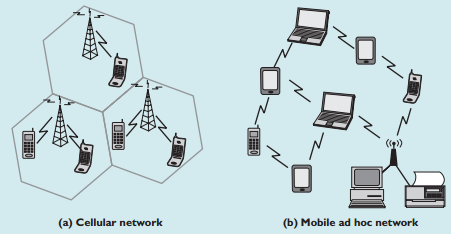
\includegraphics[width=0.8\textwidth]{adhoc.png}
     \caption [Cellular network vs. MANET]{\textbf{Cellular network vs. MANET}. This figure illustrates the difference between a regular cellular network and a mobile ad hoc network \cite{adhoc2}.}
\label{fig:adhoc}
\end{figure}

\subsubsection{MANETs} Mobile ad hoc networks (MANETs) are networks that does not rely on an underlying and fixed infrastructure (access points and routers), in other words infrastructureless. MANETs acts in a shared wireless media \cite{adhoc}. The structure of these networks change dynamically, and key factors for MANETs is self-configuration and self-organization. The members of the network are mobile and are free to join or leave the network \cite{adhoc2}, and therefore these factors are important. MANETs are based on multi-hop forwarding. This means that each node acts not only as a host, but also as a router. The nodes themselves establishes and maintain routes, and forward packets to other nodes if necessary. This enables communication between nodes that are originally not within each other's send range \cite{adhoc2}. Because of these characteristics MANETs is suited for use in situations where there are no fixed underlying infrastructure. MANETs can operate as a stand-alone solution, but it can also be attached to the Internet. This makes room for numerous of services. 

\begin{figure}[h!]
  \centering
    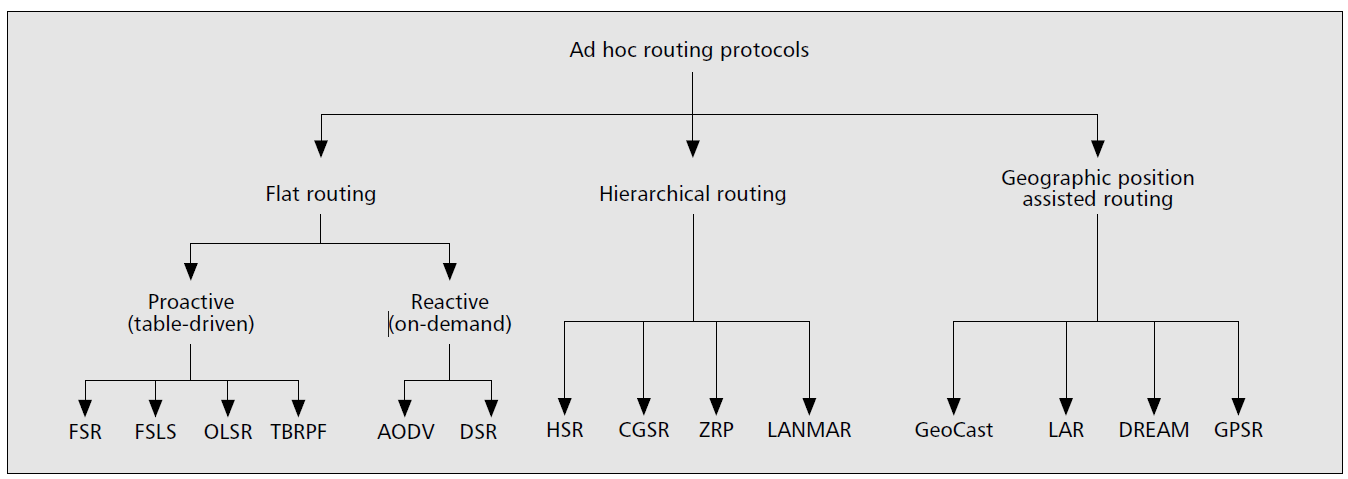
\includegraphics[width=1\textwidth]{adhocprotocols.png}
     \caption{Different groups of ad hoc routing protocols \cite{adhoc}.}
\label{fig:adhocprotocols}
\end{figure}


\subsubsection{Routing Protocols}
There exists many challenges when it comes to these types of networks. The routing protocols must be able to adapt quickly due to the topology changes. \fref{fig:adhocprotocols} shows the different groups of the ad hoc protocols that exist. The routing protocols must not cause excessive overhead. Under the category flat routing, there are two types of routing protocols; proactive and reactive. \textit{Proactive routing protocols} (e.g. OLSR) are table driven \citep{proactivereactive}. This means that every network node has a routing table for the forwarding of data. To obtain stability, each node broadcasts and modifies the routing table periodically. Proactive routing protocols are suitable when there are few nodes in the network. Because of the routing table that is periodically updated, the overhead exceeds the desired value when there are a high number of nodes in the network. In contrary to the proactive routing protocols, \textit{reactive routing protocols} (e.g. AODV) are on demand. Since they are on demand, the overhead is significantly lower. These protocols utilizes flooding. The network is flooded with the route request (RREQ) in order to set up the route. The reactive routing protocols does not have a up-to-date routing table like proactive routing protocols \cite{proactivereactive}. Routes are only set up to nodes they communicate with, and these routes are only kept alive while they are needed  \cite{adhoc2}. As shown in \fref{fig:adhocprotocols}, there are several different protocols under proactive and reactive. 

\paragraph{B.A.T.M.A.N}
Better Approach To Mobile Adhoc Networking (B.A.T.M.A.N) is the routing protocol utilized in the networks formed by the Mesh Potatoes. B.A.T.M.A.N is a proactive routing protocol for wireless ad hoc networks. This includes MANETs \cite{batman}. This protocol was developed as an alternative to OLSR (Optimized Link State Routing) \cite{batman2}. Like mentioned before, routing protocols must be able to adapt quickly to topology changes. B.A.T.M.A.N was made to be a more efficient routing protocol in this area. 

Information about the nodes that are accessible via single-hop or multi-hop are maintained and updated. 


%Eksempel på nettverk

\subsection{OpenWrt}

\section{The Cost Structure and Revenue Model(s) of Village Telco Today}

\section{Comparison of Village Telco and Other Telcos}

\section{Refugee Camps}
\subsection{The Existing Communication Methods}
\chapter{Refugee Camps}
\label{chp:refugeecamps} 

\section{Refugee Camps}
%Generell fakta

Women are in general in a more vulnerable position when living in a  camp, especially if they are single mothers. They may be solely responsible for taking care of the children in addition to sick and elderly family members, maintaining the household, preparing food, acquire water, and securing firewood. Collecting firewood for cooking is a necessity, but it forces women  to walk far away, hence making them vulnerable for sexual assault. they have to turn to sex and other unhealthy and dangerous means in order to survive. \cite{womenRefugee} 


The means of communication vary greatly in the different camps. Some have internet connection and satellite TV, other barely have access to a radio. Even though radios are the most common media for communication, it is not given that all citizens in a camp have access to one. Often people would gather around the few radios that exists in a camp. One issue that limits the usage is the batteries. They are very expensive and hard to acquire. The women were interested in news regarding their place of origin. 

Information walls and word of mouth is often used in order to spread practical information within the camp and about camp activities. Word of mouth is also used in order to retrieve information about the world outside the camp. People visiting the camp were used as sources for information. Earlier studies have shown that social connections with neighbours works as an important medium to transport information, resources and services between individuals. These kind of networking have been used to find lost family members in big camps, as well as get financial help from abroad \cite{womenRefugee}.  



\paragraph{Cell Phone}
The use of cell phones are increasing. Even though the prises are extremely high it does not stop people from calling relatives in Europe and other places in the world. 
\cite{womenRefugee} 


\section{Statistics}
When we talk about refugees it is important to divide between different types of refugees, mainly a refugee and an IDP. 

\paragraph{Refugee.} The definition of a refugee is a person who have been forced to leave their home country because of war, violence or persecution. A refugee often has a justifiable fear of persecution for reasons as religion, political opinion, race, nationality or membership in a certain social group. For these reasons are not able to, or are afraid to  return to their home country. The leading reasons for refugees flee their home country is war and ethnic, religious and tribal violence \cite{refugeeDef}.

\paragraph{Internally Displaced Person.} An internally displaced person (IDP) is a person that has been forced to leave their home and village for some reason and are a refugee in its own country. The man distinction between an IDP and a refugee is that the person has not crossed any country borders. Unlike refugees, the IDPs are not protected by any international laws nor are able to receive many types aids. in the last years the number of IDPs have drastically increased, mostly due to the conflicts between countries. 

A stateless person is someone who does not have citizenship in any country. a citizenship is a legal bond between an individual and the government in that country. 

By the end of 2012 45.2 million people were displaced by force. According to UNHCR is this the largest number in 20 years. The report show that 55 \% of the registered refugees came from countries affected by war as Syria, Afghanistan, Sudan, Iraq and Somalia. The crisis in Syria has been a major factor to displacement, the whole of 647,000 people have be forced out of the country \citep{UNHCRstat}.

In 2012 UNHCR registered 21,300 individual asylum applications from children that either were unaccompanied or separated from their family. 


\section{Interview with CARE - Dadaab Refugee Camp}
We got in contact with Mary Muia from CARE. She is a program assistant at CARE International in Dadaab, Kenya. We sent her a questionnaire with questions about Dadaab refugee camp, with focus on means of communication. The following paragraphs contains information both from different articles referred to in the text, and from the questionnaire. See Appendix \ref{chp:appendixA} for the full questionnaire. Dadaab is the largest refugee camp in the world, and is located in Daadaab, Kenya \cite{dadaab}. It was created in 1991 \cite{dadaabcare}. Dadaab was created by the government of Kenya and UNHCR to host Somali refugees displaced by civil war. Over the years, the camps have also hosted other nationalities, from the Horn of Africa, the Great Lakes and East Africa regions. These people constitute less than two percent of the camp population. In April, 2013, there were 423,496 registered refugees in the Dadaab camps. 51 \% of these were female and 58 \% were younger than 18 years old. Also in 2013, UNHCR and its partners decided to conduct a verification exercise to ascertain the current population. The reason for this was that many of those who had arrived in 2011 due to the famile had returned home. As at February, 2014, the current population stands at 369,294. The lead agency for this camp is the UN High Commission for Refugees (UNHCR) \cite{dadaab}. In addition to UNHCR, major international humanitarian agencies like Care, Save the Children and the International Rescue Committee  are active helpers in the Dadaab refugee camp. These agencies provide the refugees with critical services (e.g. food, housing, sanitation and medical help). This is an extremely challenging task in refugee camps, especially when they reach this size. During the recent years, the terror group Al Shabaad (Somali-based) have intensified their misdeeds in and around the Dadaab refugee camps. This has made the situation even tougher for the refugees and the relief agencies. 
Muia states that the biggest challenges in the camps are lack of enough space to accommodate everyone, and lack of enough funds to take care of alle the needs of the refugees. Another challenge is the language barrier between the humanitarian staff and the refugees. Many of the staff members do neither speak nor understand the Somali language, and as many as 95.6\% of the refugees are Somali. 


Muia explains how the registration process is handled. When a new refugee enters the camp, the refugee reports to a UNHCR reception desk. There the refugee is given a temporary registration, while pending full registration. Upon arrival, the refugees are given information about available services, and which agency is handling what service. Immunizations, medical attention, emergency food supply, tarpaulins, sleeping mats, jerrycans for fetching water and kitchen sets are issued to new arrivals. This is to help them start their new lives in the camp. 

To improve the situation in Dadaab, communication is crucial. In 2011, a group consisting of people from NetHope, Inveneo and the USAID Global Broadband and Innovations Program gathered to discuss ways to improve the means of communication in Dadaab \cite{dadaab}. NetHope is a consortium of over 30 international Non-Governmental Organizations (NGOs) \cite{nethope}. NetHope works with improving connectivity, with the help of information technology, among relief agencies. The aim of this project, called DadaabConnect, was to bring forward more reliable Internet, and find ways for agencies to communicate better internally \cite{dadaab}. The group put together teams that travelled to Kenya to investigate the conditions in the refugee camps, and to find out what they could implement. It was clear from the feedback they got that a better communication system was needed, and that it would make the humanitarian work much easier. It would improve the coordination and the security in the camps. Improvements of these aspects gives the humanitarian agencies better working conditions, and makes it easier for them to help the refugees with critical services. Inveneo started working with Cisco's Tactical Operations (TacOps) to install and configure a local high-speed network \cite{dadaabinveneo}. They also entered a partnership with a local Kenyan mobile and landline telecommunications service provider called Orange. The reason for this was that they wanted to extend the Dadaab compound with new data services. This could be done by using Inveneo's long-distance Wi-Fi solutions. The data services that were added included services requested from the Dadaab aid community. "DadaabNet", a high-speed network, was created in cooperation between Inveneo and TacOps. This network connected the NGOs locally, and made it possible for the agencies to easier communicate internally (VoIP telephony, file sharing etc.). Following this, in March 2012, they started the training of technicians. These technicians were people from Orange, from the technical staff of the NGOs and from Inveneo's staff. The training took place both in classrooms and in the field, in order to give the technicians a wide understanding. The results from DadaabConnect has been great. The humanitarian agencies has gotten better working conditions, due to the improvements in means of communication. Other positive outcomes is that the network is more reliable and cost effective. 

Muia did not specifically mention this project in her answers, but answers on our questions about means of communication within the camp, and with the outside world. She states that CARE as an organization has invested in communication systems in cooperation with ISPs in the capital city of Kenya, Nairobi. Through this cooperation the camp staff are assured to get access to Internet for both official and social use. Several Kenyan telecommunication companies have put up equipment in the camp area, and the camps are therefore provided with access to mobile communication and Internet. Although this is set up, Internet and telephone service outages are fairly common. In addition to mobile communication and Internet, there are radio station services and access to digital television. CARE use telephone services to reach out to refugee staff. 50\% of the refugees have access to mobile phone services. Posters an radio is also used to reach out. Word by mouth (e.g. over speakers) is also a communication technique employed. There are two main telecommunication providers in Dadaad, hence little competition. This makes the prices higher. We asked Muia how the refugees can afford having their own mobile phone, when the costs are high. She says that many refugees have been in the camps for a long time, and therefore have had the time to establish small businesses which gives them some profit. While others get money sent from their relatives. 


\section{Interview with Norwegian Refugee Council}
%hun mener vi skal klassifiere for oppgaven sin del av vi snakker om offisielle leirer. UNHCR har ansvar da. Monitirere enklere da om de tingene er på plass, og evt. hva slags system de bruker. 

We had a Skype interview March 12, 2014, with Katrine Wold from the Norwegian Refugee Council (NRC). The aim of the interview was to hear a little bit about her work in refugee camps and how the situation in the refugee camps are today, with main focus on means of communication.
Katrine Wold has been working for NRC for many years, and also has a background from United Nations (UN). She has worked in emergency and crisis situations abroad. She is specialized in camp management and coordination. In recent years she has been responsible for education, and have had the main focus on youth. We asked her which refugee camps NRC is working in, but she could not give us a clear answer on that question. The reason for this is that NRC works in over 24 countries, and have, as of 2013, reached out to 4.4 million people. She makes it clear that there are a difference between internally displaced persons (IDPs) and refugees. An official refugee must cross a boarder, or else you are internally displaced. NRC works both with refugees and IDPs, and also with people who are affected by having refugees in their local area. NRC does not only help with operational issues in the camps, but they mainly offer services the refugees need. When dealing with refugees there exists international laws and regulations. These also states what kind of human rights exists. Everyone have rights! The vast majority of countries have ratified the UN refugee commission, which has been formed by the international society, UN, and authorities via UN's forums. The commission is an important premise when working with refugees. It is important to know which rights you have as a humanitarian worker, and which rights the refugees have. 

We ask her about how communication within the camp is conducted. She takes Kenya as an example. NRC has been working in the largest refugee camp in the world, Dadaab Kenya, for many years.  Some have the main responsibility for what is going on in the camp, and that is the  authorities. They often ask the international community (e.g. NRC) for help. Wold states that it is then important to establish good communication and information flow between the ones working in the camp (the different organizations). This communication takes places by either establishing coordination meetings and by other types of mechanisms. These meetings includes the relief organizations working in the camp, and the authorities. The goal is not to make a permanent home for the refugees, but that it is safe when they are in the camps and that they move on (either go home or find another place to live). Living in camps is a temporary life situation. She states the different types of communication; internally between the workers in the camp and communication with the refugees. It is important to establish open transparent coordination mechanisms, in other words ensure good forums where the refugees can communicate and inform the workers in the camp what their needs are. This can only be achieved by recognizing that refugees is not a large mass, but individuals with different needs and different life situations. The humanitarian and authorities try to establish some sort of local elections. This means that the refugees can choose representatives who's job is to be in communication with the primary humanitarian managers in the camp. The reason for this is that it is impossible for the humanitarians to talk to 500 000 people. The communication between the representatives and the managers be done either through meetings, or in an informal manner. Overall, this creates a communication pattern in the refugee camps. Wold states that there a few places without mobile coverage, and that the majority of the refugees have a mobile phone. Mobile phones are used frequently in terms of distribution. Mobile phones are often used as a tool when goods (access to money, food etc.) gets distributed to the refugees. They can "add credit" to their card, and use this as "payment". This an up-and-coming way of doing distribution. Mobile phones are also used to collect information, for example by sending the refugees surveys on their mobile phone. 


In general, Wold states that methods of communication can be via mouth, radio, billboards, data communication, but this all depends on which camp and what is allowed in the camp. The law in the refugee camps depends on the national authorities. In some camps it is allowed to establish a data communication center, but in other camps this is illegal. It is important that when the refugees arrive to a camp that they get informed of the current situation, and what rights they have. The distribution of this information takes places primary by someone called the camp management agency. They have the daily coordination responsibility for what is going to take place in the camp. It must be made clear to the refugees where they can obtain different types of services, and also what is expected of the refugees. It is important that the refugees at an early stage get the opportunity to contribute positively in the camp, or else they can end up with something called "dependency syndrome" (they feel incompetent and get totally dependent on external assistance). 

Another question we asked her is how the refugees get registered in the camps. Here she states the importance of distinguishing between official and unofficial camps. The definition of a camp is that people are gathered together and live there. Registration is done in official camps, and then there are someone who is responsible for the operation of the camp. When refugees are registered they get an ID card. This ID card is very valuable, because it indicates that you, as a refugee, have access to the goods that are available in the camp. The registration procedures can vary, but most often there exists computer systems for the registration.



\chapter{Main Work}
\label{chp:quickrollout} 

Make a best practice for quick roll out, by the use of a MultiBox. 

*Alt som står på norsk er kommentarer på hva mer som skal være med.

*Her skal det være en mer utfyllende innledning til kapittelet. Hva kap. inneholder.


\section{Set-up of the Mesh Potatoes}
The set-up of the Mesh Potato is a process including installing firmware, allocating IP-addresses, providing Internet to the network and so on. The firmware used for the Mesh Potatoes is called Small Enterprise/Campus Network (SECN) Firmware \cite{ChoosingFirmware}. A flashing process is applied in order to install/update the firmware on the Mesh Potato. See the SECN User Guide in Appendix \ref{chp:appendixB} for a more detailed description of how to set up the Mesh Potatoes and how different networks can be built. 

\subsection{Installing Firmware on Mesh Potato 1.0}

The flashing process is the process of updating or changing the firmware (SECN) on the Mesh Potato. We updated the firmware by using the potato-flash application \cite{flashing}. This is a specialised software application for the Mesh Potato. Potato-flash can be used regardless of previously installed firmware on the Mesh Potato \cite{InstallingSecnFirmware}. 

\begin{enumerate}
\item Downloaded the 64 bit potato-flash utility from \url{http://download.villagetelco.org/utilities/potato-flash/potato-flash-64bit/} to the folder \textbf{/etc/local/bin}.
\item Made the potato-flash file executable by writing \textbf{cmod +x /usr/local/bin/potato-flash-x64} in the Linux terminal.
\item Downloaded the rootfs (openwrt-secn1_1-GA01-MP01-root.suashfs) file and the kernel (openwrt-secn1_1-GA01-MP01-vmlinux.lzma) file from \url{http://download.villagetelco.org/firmware/secn/stable/mp/SECN-1.1/} to a folder we called mp\_firmware on our local directory.
\item Opened the terminal and wrote the following commands: 
\end{enumerate}


\begin{framed}
\noindent \textbf{Root environment:} 
\begin{lstlisting}[language=bash]
  $ sudo su
\end{lstlisting}

\noindent \textbf{Turn of network manager:}
\begin{lstlisting}[language=bash]
  $ service network-manager stop
\end{lstlisting}

\noindent \textbf{Bring the interface connected to the MP up:}
\begin{lstlisting}[language=bash]
  $ ip link set eth0 up
\end{lstlisting}

\noindent \textbf{Go into the directory containing the .squashfs and .lzma files:}
\begin{lstlisting}[language=bash]
  $ cd <the directory containting the .squashfs and 
  .lzma files>
\end{lstlisting}

\noindent \textbf{Assign IP-address to the interface:}
\begin{lstlisting}[language=bash]
  $ ifconfig eth0 1.1.1.1
\end{lstlisting}

Before running the potato-flash utility we made sure that the Mesh Potato was unplugged from the power and that the Mesh Potato was connected to your PC via an Ethernet cable. 

\noindent \textbf{Executing the potato-flash utility:}
\begin{lstlisting}[language=bash]
  $ potato-flash-x64 openwrt-secn1_1-GA01-MP01-root.suashfs 
   openwrt-secn1_1-GA01-MP01-vmlinux.lzma
\end{lstlisting}
\end{framed}

Briefly after the potato-flash had been executed, dots stared appearing on the screen, like shown in \fref{fig:flashing}. When these dots started appearing, we plugged the power supply back into the Mesh Potato. 

\begin{figure}[t]
  \centering
      \includegraphics[width=1\textwidth]{flashing}
  \caption [Flashing the Mesh Potato]{\textbf{Flashing the Mesh Potato.} This figure shows the flashing process from when we first flashed our Mesh Potato 1.0}
  \label{fig:flashing}
\end{figure}


\subsection{Installing Firmware on Mesh Potato 2.0}
*Her skal vi skrive om flashing prosessen, hvordan få internett til nettverket, hvordan  en MP kan koble seg til de ulike uplinkene, 3G via TP-links til mesh nettverket (?). 
%Flashing process
%How did we get Internet to the network?
%Hvordan en MP kan koble seg til de ulike uplinkene?
%3G via TP-links til mesh nettverket?

\subsection{Example Mesh network}
We first started experimenting with the Mesh Potatoes by setting up a small network consisting of two MPs connected to each their plain old telephone, and a computer running Ubuntu Linux. This simple network is shown in \fref{fig:network}. Each of the MPs were assigned a static IP address, these addresses were not part of the LAN address space. The IP addresses are allocated in a predefined default address space 10.130.1.xxx. To administrate the MP devices we used a workstation linked together with one of the MPs in the network by using a Ethernet cable (can also be connected via Wi-Fi). We assigned the workstation a static address within the same address space as the MP devices. We were able to make phone calls between the Mesh Potatoes by dialling the last octet or the whole IP address.

\begin{figure}[b]
  \centering
      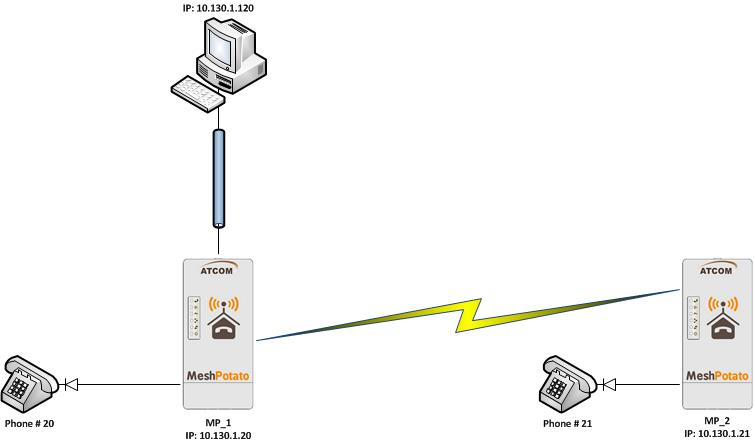
\includegraphics[width=1\textwidth]{network1}
  \caption [Example of a simple mesh network]{\textbf{Simple mesh network.} This figure illustrates a simple mesh network with the use of Mesh Potatoes.}
  \label{fig:network}
\end{figure}

\subsection{The SECN Web Interface}
Village Telco provides a SECN web interface for configuration and management of individual MPs. This web interface can be accessed by entering the IP address of the MP in a browser. In order to be able to do this, the PC must be on the same subnet (exact same prefix) as the MP.  









\section{The Emergency Box}
We want to make an emergency box that has high adaptability, so it can be utilized in several different scenarios. 

*Mer utfyllende introduksjon til nødboksen  

\paragraph{Previous/similar work}
Something similar has been done before by Keith Williamson, a volunteer in the Village Telco community. His idea of utilizing the Mesh Potatoes in emergency situations started with his interest in amateur radios for use in emergency situations. He sat together a "go box" by using a waterproof Pelican 1200 case.  This case contained a bracket holding the Mesh Potato, a rechargeable Li-Ion or Li-Poly battery, telephone handset, and to connect it all together and get a on/off switch, a junction box was included \cite{keith}. 

*Se om vi finner minst et eksempel til på noe lignende som er gjort før. 

*Hvordan er vår boks annerledes fra Keith sin, hvordan er den satt opp, hvordan er den laget, hvordan fungerer den, forklare ulike komponentene, forklare endringer som gjøres underveis grunnet testing (flere versjoner), ting som gjøres for at den kan rulles ut raskt (feks script). 
%Hvordan er den annerledes fra Keith sin?
%How is the box set up?
%How is it made?
%How does it work?
%Explain the different components
%Explain evt. changes
%Script?

\subsection{The Different Components}
The components of our emergency box is described in \tref{tab:components}. 

\begin{center}
\begin{table}[!hb]
\caption{\label{tab:components}The components of MultiBox}
    \begin{tabular}{ | l | p{9cm} |}
    \hline
    \textbf{Component} & \textbf{Description and purpose} \\ 
    \hline
    Mesh Potato &  \\ 
    \hline
    Suitcase/box &  A suitcase made of high quality plastic coated with aluminium foil. Strengthened edges and corners of aluminium and steel. It has a soft-padded interior, than can be split into different rooms. Two snap locks with keys, and a solid handle for carrying. Dimensions: 455x330x152 (width, depth, height). Weight: 2,6 kg. \\ 
    \hline
    Power supply & A gel battery (12 V and 5 Ah). No need for maintenance. The battery acid is bound in a viscous gel. This prevents leakage, even when the battery is mounted horizontally. Long lifetime and safe to handle. The battery is fully closed, and do not need refill of battery water. No hydrogen gas or other gas might leak. When the battery is charging no gas or acid vapor is emitted, hence the battery can be placed in narrow or enclosed spaces. The battery withstands multiple discharges. The gel battery is ideal for seasonal or occasional use, since it have a slow self-discharge tempo, and a good ability to recover after deep discharging. Dimensions: 114x69x109. Weight: 2,16 kg. \\
    \hline
    Plain old telephone & \\
	\hline
	Junction box & \\
	\hline
	Solar panel & Solar panel from Multicomp with item number: MC-SP10-GCS. Power rating: 10 W. Power Voltage Max: 17 V. Dimensions: 357x280x18\\
	\hline
	Charging regulator & Regulator for 12 V solar panel. Protects the battery from overcharging and discharge. The charging regulator is connected between the solar panel and the battery to regulate the voltage to the battery. Capacity: 100 W / max. 7 A. Overcharging protection: 14.5 V. Discharge protection: <10,5 V. Three diodes shows charging, high voltage and low battery voltage. \\
	\hline
    \end{tabular}
   \end{table}
\end{center}

\subsection{Battery and Charging Calculations}
All the calculations done in this section is based on the equipment described in \tref{tab:components}.

\paragraph{Charging with solar panel.}
How long it will take for the solar panel to charge the battery from fully discharged to fully charged depends on how much sun there is, but with the peak value of the solar panel (10 W) it takes: 

The solar panel capacity is:
$$Amp = \frac{Watt}{Volt} = \frac{10 W}{17 V} = 0.59 Ampere$$

If the battery is completely discharged it will take: 

$$Amp\times Hours = AmpHours \Rightarrow Hours =\frac{AmpHours}{Amp} = \frac{5 Ah}{0.59 A} = 8.47 Hours$$

to fully charge it. 

\paragraph{With Mesh Potato v1.0}
With the components described in \tref{tab:components} the number of hours the MP1 can last with fully charged battery is: 

$$Amp = \frac{Watt}{Volt} = \frac{2.5 W}{12 V} = 0.208 Ampere$$
$$Amp\times Hours = AmpHours \Rightarrow Hours = \frac{AmpHours}{Amp} = \frac{5 Ah}{0.208 A} = 24 Hours$$

\paragraph{With Mesh Potato v2.0}
With the components described in \tref{tab:components} the number of hours the MP2 can last with fully charged battery is: 

$$Amp = \frac{Watt}{Volt} = \frac{? W}{12 V} = ? Ampere$$
$$Amp\times Hours = AmpHours \Rightarrow Hours = \frac{AmpHours}{Amp} = \frac{? Ah}{? A} = ? Hours$$

\subsection{The Process of Quick Roll-Out}
*Forklare spesifikke ting som er tatt i betrakning for å gjøre utrullingen raskest mulig. Feks scripting, manual etc. 

*Hvordan utdele telefonnummer raskt, opplæring av folk, 


\section{Up-Link}
Our main focus when deploying the emergency boxes, is to provide Internet to the mesh network. This is because it is crucial to have the possibility to communicate with the local community and the outside world during an emergency situation. In 2011, UN declared Internet access a human right \cite{HR}. This says something about the extent of the Internet, and the importance of connectivity. In order to provide Internet to the mesh network formed by the emergency boxes, at least on the the Mesh Potatoes must be connected to an access network via an uplink. An uplink connects a device or a LAN to a larger network \cite{uplink}. Which type of access network that is available depends of the location. Some places there might exist a stable landline, other places not. Then an option could be to use satellite or cellular networks. It is therefore important that the emergency box has high adaptability in order to fit different scenarios. The availability of the different uplinks is not the only thing that vary. The up-link speed and the price also varies from place to place, but also varies between the types of uplinks. In the following sections, we will look at some of the uplinks available, and how Internet access can be provided to the mesh network.  

\subsection{Internet via Telephone-line}
The most common way of getting Internet access is via a landline. The telephone lines are most often used for this, since they can be converted to broadband. In this way it can be used for phone calls and Internet simultaneously \cite{internet}. The line is usually in the form of twisted pairs (copper lines). These lines support broadband up to 10 Mbps, and are often in form of ADSL, or other digital subscriber line of type x (xDSL) technologies \citep{audestad}. Internet via telephone lines can be provided as a stand-alone solution, or it can be provided together with television or/and phone service. The latter option is usually cheaper. Internet through landlines have a high reliability \cite{cablevssatellite}. We will now shorty describe some technologies for getting Internet access via a telephone line; dial-up Internet connection, ISDN, and DSL. Although dial-up Internet connection is practically extinct in developed countries, we will include it here due to the different application scenarios for the emergency box. 

\paragraph{Dial-up Internet connection}
Dial-up is an analogue technology that utilizes the telephone line. A telephone wall jack is used as a fixed point of connection, and the computer is connected to a voiceband modem. With this technology, the data is transmitted over the same frequencies used for phone calls. Hence, if you only have one telephone line, you cannot take a phone call and use Internet at the same time \cite{differentuplinks}. Along with the digital era, better internet technologies were introduced; ISDN and DSL. 

\paragraph{ISDN}
Integrated Services Digital Network (ISDN) is a fixed internet connection, which also utilizes the telephone lines. When using ISDN, as with dial-up, a telephone wall jack is used as a fixed point of connection. But ISDN utilizes a ISDN terminal adapter instead of voiceband modem. This ISDN terminal adapter sends out digital signals. The data speed varies between 64 Kbps - 129 Kbps. The speed of the data is symmetric, which means upstream and downstream data rates are the same. In contrary to dial-up, ISDN allows voice calls and transmission of data simultaneously. ISDN is faster than dial-up, but the speed is nothing compared to the speed obtained using DSL \cite{differentuplinks}. 

\paragraph{DSL}
Digital subscriber line (DSL) is, like the name indicates, a digital high-speed technology for Internet access that allows simultaneous voice and data transfer. Like dial-up and ISDN, DSL also run over the telephone lines. With DSL the data is not converted between analogue and digital signals. Despite this, the signals are modulated in order to be transferred on non-voice frequencies. DSL is an always-on technology, and differ from the previous technologies mentioned in this way. Only a small part of the telephone line is used for voice signals. The DSL technology allows utilization of a unused frequency spectrum of an telephone line, hence making it possible to transmit data faster. When the voice and data signals arrive at the telephone company's local switching station, they are separated and routed differently; voice to regular telephone system and data to the ISP, and then the Internet. A connection must be within approximately 5 kilometres of a station in order for DSL to work. The speed depends on many factors. Data can be transported up to 6 Mbps (distance of approximately 2 kilometres). Relevant factors that have an impact on the speed is distance to the switching station and the quality of the telephone line. Like mentioned earlier, there are different types of DSLs. The most common is ADSL, where the A stands for asymmetric; the downstream speed is faster than the upstream speed \cite{differentuplinks}.

\subsubsection{Quickly Connect the Emergency Box to This Uplink}
*Forklare hvordan man raskest mulig kobler nødboksen til akkurat denne type uplink.

\subsection{Cellular Network Technologies}

\begin{figure}[b]
  \centering
      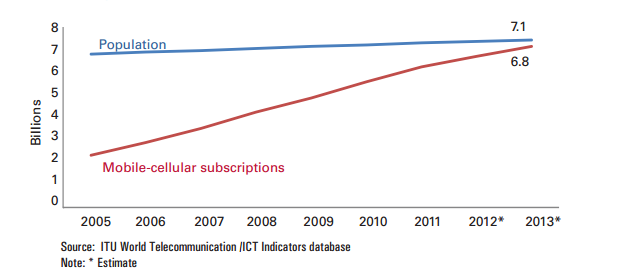
\includegraphics[width=1\textwidth]{mobilesubscriptions.png}
  \caption [Number of mobile-cellular subscriptions]{\textbf{Number of mobile-cellular subscriptions} The figure shows that the growth of mobile-cellular subscriptions have increased drastically during the last decade, and show that there are almost as many as there are people in the world \cite{itu2013}.}
  \label{fig:subscribers}
\end{figure}

%ITU2011-artikkel
It is getting more and more common to use cellular technologies for broadband. Around 2011 number of mobile-broadband subscriptions grew to twice as many as the number of fixed-broadband subscriptions. In developed countries it is common to have a fixed-broadband connection, and use a mobile-broadband network in addition to the fixed. In developing countries on the other hand, it is not a given that there is access to a fixed-broadband connection. Then mobile-broadband can be the only method of access available. In 2011, 90 \% of the world's population had 2G coverage, and 45 \% had 3G coverage \cite{itu2011}. By 2013, the number of mobile-cellular subscriptions had reached a high level, and were approaching the number of people in the world, like shown in \fref{fig:subscribers}. From 2011 to 2013, the number of mobile-broadband  subscriptions more than doubled in developing countries \cite{itu2013}. 

Through mobile network technologies, high-speed Internet access can be provided via portable devices. In order to get mobile broadband, there must be a cellular network (GSM, CDMA) service available. The key technologies when talking about mobile broadband is 3G and 4G (respectively third and fourth generation wireless networks) \cite{mobilebroadband}. With 3G the average speed is 0.5 to 1.5 Mbps, and with 4G the average speed is 2 to 12 Mbps. These vary, due to different versions of each technology, underlying service etc.. And like with everything else, the actual and realistic speed differ from the peak speed \cite{3gvs4g}. 

\subsubsection{Quickly Connect the Emergency Box to This Uplink}
*Forklare hvordan man raskest mulig kobler nødboksen til akkurat denne type uplink.


\subsection{Satellite}
%ulovlig i feks india, hva skjer da? http://en.wikipedia.org/wiki/Satellite_phone
Internet from satellites are offered by a satellite Internet provider \cite{cablevssatellite}. The satellite are orbiting the Earth, and get signals from a land based Internet connection. To get Internet broadband via satellite you need a satellite dish. The main advantage of using satellite is that it provides an universally available Internet access \cite{broadband}. Since it is universally available, it is fitted for use in rural regions where there exists no landlines or other options for connecting to the Internet. But like with everything else, there also exists disadvantages with using satellite-Internet. Since it is a shared medium, privacy concerns arise, and the speed are dependent of simultaneous use. Also the connection can be affected by bad weather, unlike for a wired connection, hence it is not as reliable as cable. 

\subsubsection{Quickly Connect the Emergency Box to This Uplink}
*Forklare hvordan man raskest mulig kobler nødboksen til akkurat denne type uplink.

\subsection{Summary Up-Links}

\begin{center}
\begin{table}[!h]
\caption{\label{tab:uplinks}Advantages and disadvantages - Up-links \cite{comparisonuplinks}.}
    \begin{tabular}{ | l | p{4cm} | p{5cm} |}
    \hline
    \textbf{Up-links} & \textbf{Advantages} & \textbf{Disadvantages} \\ 
    \hline
    Landline/xDSL & High reliability, cost effective, good speed. & Low availability in rural areas. \\ 
    \hline
     Cellular networks & High availability, fitted for "on the move"-use. & Expensive, slower than xDSL.\\
    \hline
    Satellite & High availability.  & Unreliable, expensive, slower than landline.\\ 
    \hline
    \end{tabular}
   \end{table}
\end{center}

*Forklare ulikhetene og likhetene ved å koble nødboksen til de forskjellige uplinkene. 

\section{Future Internet Access Methods}
Different methods of distributing Internet is always under development. The previous up-links described is well established, but in many parts of the world not fully developed or not affordable to the average person. The large technology companies, like Google, are experimenting with different ways of distributing Internet. 

\subsection{Google's Internet Balloons}
The majority of the world today is not connected to the Internet. Two thirds of the worlds population does not have access. Project Loon, a Google project, is a network of high altitude balloons travelling in the stratosphere, and through this network be able to give Internet to the Entire world. Cost effective, reliable and inexpensive internet connection to everybody. The project started in June 2013 as a experiment in New Zealand \cite{loon}. 

\begin{figure}
        \centering
        \begin{subfigure}[t]{0.43\textwidth}
                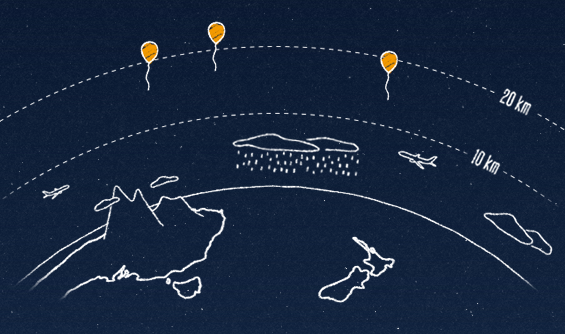
\includegraphics[width=\textwidth]{loon2.PNG}
                \caption[The Balloons are situated in the stratosphere]{\textbf{The Balloons are situated in the stratosphere.}} 
                \label{fig:loonStratosphere}
        \end{subfigure}%
        ~ %add desired spacing between images, e. g. ~, \quad, \qquad etc.
          %(or a blank line to force the subfigure onto a new line)
        \begin{subfigure}[t]{0.415\textwidth}
                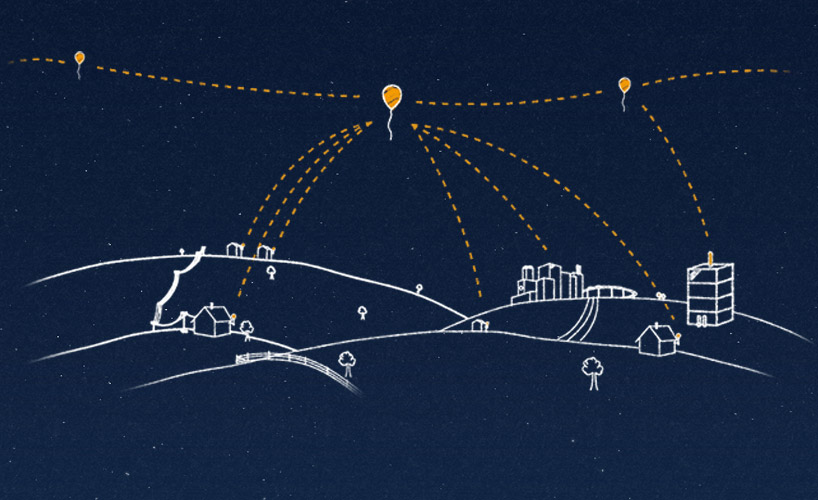
\includegraphics[width=\textwidth]{loon1.jpg}
               \caption[Connecting to the Internet]							{\textbf{Connecting to the Internet}} 
                \label{fig:loonConnect}
        \end{subfigure}
        ~ %add desired spacing between images, e. g. ~, \quad, \qquad etc.
          %(or a blank line to force the subfigure onto a new line)
        \caption{Project Loon: Balloon-powered internet for everyone.}\label{fig:loon}
\end{figure}

The balloons are 15 meter in diameter. They travel about 20 km up in the air, in the stratosphere, twice as high as airplanes and weather, this is shown in \fref{fig:loonStratosphere}. At this altitude there are many layers of wind, each varies in direction and speed. By regulating which wind the balloons are flying in it is possible to control their position, and steer them in the desired direction. \fref{fig:loonConnect} show that  people can connect to the Internet shared by the balloons by having a special antenna attached to their house. From this antenna the signal bounces to one balloon which again bounces through the other balloons and down to the Local Internet Provider on earth. This creates a network in the sky. 

In order to control the altitude of the balloon, there is a special designed control system. The system is managed remotely from the ground. By either pumping air in, or letting air out of the balloon, one can decide in what layer of air the balloon should be in. Letting air in and out is not the only way to decide is the balloon should go up or down, but it is the only way to do so in huge scale. A GPS is attached to each balloon in order to keep track of precise positions and see how the winds are changing. There are enormous amounts of data collected. The balloons are flying at the same speed as the wind.  

The balloons contains specially designed antennas and radio systems. This in order to receive signals from Project Loon only, in order to achieve high bandwidth over long distances. Satellites stay at the same place and at the same altitude. This means that the satellite dish can be mounted in the right direction. This is not the case with the balloons, they are in constant movement and they also vary in attitude. A fixed pointing dish would therefore not work. The antenna needs more sensitivity to an angle than it does straight up, which results a uniform signal strength. 

Since the balloons are in constant movement, it is important to make sure that there always is a balloon available and one ready to move in when one move out so that the connectivity always are available. If not this project would not be of much use. Every balloon contains information about all the other balloons in order to spread out nicely. Think of it as a flock of birds, they always look at the one next to them and space out nicely.

The balloons are solely run on solar power. The balloon works as a communication tower in the sky. The solar panels catches the sunlight that is available during the day, as well as charging up the lithium-ion battery to last the night. In the stratosphere it is -70 degrees Celsius, these extreme cold conditions are not ideal fro the lithium battery. In order to make sure that the battery does not loose its effective battery capacity it is important that the battery is kept warm. The battery pack is insulated to reflect the heat that comes of the electronics to stay warm. This is still under development. 

When it comes to lifetime, the goal is that the balloons stay alive for a 100 days, or 3 laps around the globe. It is important to make sure that the balloon is leak free. The material is under a lot of stress, air is constantly being pumped in and out to control the position.. As well as the extreme cold and warm temperatures. 

Both on the way up and down the air traffic control in the specific country have to be contacted since they go through airspace. Project loon requested permission to land on Norwegian soil according to Teknisk Ukeblad, a Norwegian science magazine. This permission was approved \cite{loonTU}.

The area of usage is enormous, it is everything. Situations where the Internet infrastructure has not been built out, either because it is too expensive or just not possible. Emergency situations, natural disaster and other situations where the cell towers are down and causes the need to communicate. We can also see the political aspect of it. With these balloons the Chinese people can finally have access to a free and uncensored Internet. Project Loon is still a development project with extensive testing. The project are taking into use what everybody have in common, namely the sky, to reach out to all the areas where access has not been possible. It is expensive to have enough balloons in the sky in order to have good enough coverage. Also the speed is not really high. And even though a specialized antenna is required to get access, this is breakthrough in order to get the whole world connected \cite{loonYouTube, loonNorsk}.

Although this solution is not an option for distributing Internet as of today, it could be a good option in the near future. The solution is affordable and well compatible with our emergency box solution.

*Sammenligne med lavbane satelitt (LEO), som feks Iridium

\section{Apple's Mesh Network}
In March 2014 a new iOS app was released, FireChat. This app enables the possibility to chat with people "off-the-grid" \cite{fireChat}. FireChat utilizes Apple's Multipeer Connectivity Framework introduced in iOS7 \cite{appleMesh}. Applications that communicates through this framework creates a mesh network similar to the one created by the Mesh Potatoes. 

The Multipeer Connectivity framework provides support for discovering services provided by nearby iOS devices using peer-to-peer Wi-Fi, infrastructure Wi-Fi networks and bluetooth to communicate with those services. This communication could either be message-based data, streaming data and resources such as files \cite{multipeer}. These technologies have a short range, but this range can be greatly extended by a chain of users that creates a mesh network, see section \ref{subsec:mesh} for more information about mesh networks. AirDrop is a product that have been out there for a little while and also utilizes mesh networks. The Main difference is that FireChat is fully decentralized and peer-to-peer. When there are multiple users in one area FireChat relay messages in the same way as Internet, from node to node, just in this case it is from phone to phone.  This, not only, enables two users to chat with each other without Internet connection, but also far beyond Wi-Fi and Bluetooth range from each other, using the chain of users (phones). For example if Bob is connected to Alice, and Alice is connected to Carol, Bob and Carol can send messages to each other. This chain can be indefinitely long. As long as no one device goes out of Wi-Fi range, all the devices can communicate with each other. 

This new framework will mainstream wireless mesh networking. Internet can now become available in places where it earlier was non existent. This could for example be a hotel basement, cave or rural areas where there are no cellphone towers, or disaster situations where Wi-Fi or mobile broadband  is no longer available. There are many benefits with the use of mesh networks. Mesh networks does not require a centralized infrastructure, there are no need for all the devices to be connected to a access point (as a router). Another benefit is that the mesh network is really easy to set up - everybody just uses the app FireChat (or similar applications like AirDrop), the network is created and everybody is connected. Simple as that! 

The possibilities for this feature are enormous. Both in the creation of applications but also the area of usage. In a lot of countries Internet and mobile broadband connection is extremely expensive, people might afford a used cellphone but not the cost to connect. With this new feature Internet connectivity can be spread through the mesh network needing only one node (phone) to have internet access. This way of spreading connectivity can open the possibility for people in rural, poorer areas like slums and small villages to stay connected. But not only the poor and rural areas can benefit from this new mesh-networking feature. Young people that does not have a phone can use an iPad or similar to talk to their friends. Or teens with restricted cell contracts can still connect with their friends, just with the help of the neighbours kids phone. Since FireChat enables communication without the use of internet it can be a useful tool to communicate privately and also to send sensitive data.
 
It is not only Apple that is seeing the enormous potential in main-streaming mesh networking. Google has also expressed that they are working on a home mesh network \cite{googleMesh}. FireChat and AirDrop is just the beginning. We believe more extensive and mind blowing applications are to come. 
 
\section{Different Scenarios Where a Quick Roll-out is Necessary}
%What are the specific need for the different scenarios? What adjustments are necessary?

Everyday there are situations all over the world that in some way affects the modern communications systems, or causes a need for one. These situations can range in everything from big natural disasters like the tsunami in Japan or the volcano outbreak in the Philippines, where either parts of the communication system is not functioning or there is a desperate need for one. To temporary refugee camps and IDP camps, and situations where a mobile tower is down, or blackouts. Also more festive situations can have use of the quick roll-out system. Imagine a big group gathered at a festival in another country. It is expensive to call or use mobile data, to be able to use cheap internet via the mesh Potatoes would save the users for a lot of money. 

\subsection{Natural Disasters}
%Asia og Sør-Amerika
%Philippines - contact Kenneth Bjerkelund to find out their needs for internet etc. makingchange.no. 
A Natural disaster is defined as; \textit{any event or force of nature that has catastrophic consequences, such as avalanche, earthquake, flood, forest fire, hurricane, lightning, tornado, tsunami, and volcanic eruption} \cite{naturalDisaster}.

%Hvorfor viktig å kunne kommunisere 
%grunner til at at et backupsystem er nødvendig


History shows that cellphone service is not a reliable service during an emergency situation. During 9/11 the system became heavily overloaded, and when hurricane Katrina hit 70\% of the cell phone towers where knocked down. One might think that if they live in a big metropolitan that they would be safer \cite{disasterComm}. 

These are situations in the western world. When looking at the eastern, and often less developed world, that are even more vulnerable to natural disasters, the situations are different. 

* fylle ut mer her
* Hvorfor viktig å kunne kommunisere 
* grunner til at at et backupsystem er nødvendig


\paragraph{Hurrican Sandy}
Hurricane Sandy hit big parts of the Caribbean as well as the southeast parts of the Unites states at the end of October 2012 \cite{WikiSandy}. As many as 25 percent of the citizens in the affected areas lost cell phone coverage, and even more lost electricity. Emergency communication is a challenge in natural disasters, and often leave the public with out a way to call the the emergency number, but also makes it difficult for first responders (as fire fighters, police, etc) to communicate.  Satellite is sometimes used but is an expensive solution and they have more fixed restrictions, plus the fact that the equipment needed, phones and dishes, are expensive. No single communication system is fault free, and there always have to a backup to the backup. Satellite was used but the phones are expensive and the lines can be oversaturated if others parties are trying to connect to the network at the same time. A small aperture terminal (VSAT) trailer was also used to act like a satellite ground station. Finding a good spot for the trailer can be tricky, it requires clear view to the sky and can not be placed too close to a large building. The Red Cross launched an emergency preparedness application for smartphones. The application had a peak in downloads right before the hurricane hit, but when the commercial wireless network failed, they had to back to the old way of spreading information. Distributing paper files, going from house to house to check up on peoples welfare, give information word-by-mouth and using bullhorn \cite{hurricaneSandy}.

\paragraph{Philippines}

*Skal fylles ut mer her

November 8 2013 the typhoon Haiyan, a powerful tropical cyclone, struck and devastated parts of southeast Asia, in particular the Philippines. Haiyan is the strongest hurricane in wind speed ever recorded. The hurricane have the highest number for casualties, killing at least 6,268 people in the country alone \cite{wikiHaiyan}. International humanitarians and the government at the Philippines was warned about the storm in advance, but nobody could anticipate its viciousness. Some of the first teams on the spot was the communication experts, in order to coordinate, and make sure information was spread as desired.    \cite{disasterResponse} 

Clusters are groups of UN and non-UN humanitarian organisations that specialise in emergency repons in areas such as water and sanitation, health, shelter, logistics, food security and agriculture. The cluster approach was applied for the first time after the 2005 earthquake in Pakistan \cite{disasterResponse}.


\paragraph{Utilizing the emergency box.}
*detaljert forklaring på hvordan nødboksen kan settes opp for bruk i denne type scenario. 

\subsection{Temporary Refugee and IDP camps}

*Skal fylles ut mer her

Not all refugee and IDP camps are as well established, like the ones in Dadaab. Many camps are short-term, and are therefore in more need of a temporary communication system. In this case, setting up Mesh Potatoes in the camp to provide the refugees/IDPs with Internet access is an option. 

\paragraph{Utilizing the emergency box.}
*detaljert forklaring på hvordan nødboksen kan settes opp for bruk i denne type scenario. 

\subsection{Festivals}
Image you are at a music festival with your friends in a foreign country. There are thousands of people, and much activity. In a scenario like this there are many reasons why an Internet connection would be beneficial. You could loose your friends, have to inform your friends about something urgent, inform the staff if an emergency situation occur and so on. Since it is very expensive to send text messages/make phone calls or use mobile networks when you are abroad, it could be an idea to use Mesh Potatoes to provide the people at the festival with Internet access. This could be set up by the organizers in advance. Although this adds an extra cost to the organizers, the people attending the festival can save a lot of money by refraining from using the expensive services available on their cell phones. The organizers could add an extra fee to prize of the festival pass, and it would probably still be beneficial for the people at the festival. 

\paragraph{Utilizing the emergency box.}
*detaljert forklaring på hvordan nødboksen kan settes opp for bruk i denne type scenario. 

\subsection{Breakdown of Mobile Towers}

The 10th of June 2011 one of Telenor had problems with one of its servers in Oslo. This problem caused a down time of 18 hours and affected 3 000 000 Telenor users \cite{listeNedetid}. Not only was this the biggest problem Telenor have had since they opened their mobile network in 1993, but also the longest downtime and highest number of affected users recorded in Norway. In addition to this it all happened in a period with severe flooding in big parts of the eastern Norway, and made it difficult to reach emergency numbers. The fact that the problems occurred during the flooding just made the situation much worse \cite{TelenorNede}.

\paragraph{Utilizing the emergency box.}
*detaljert forklaring på hvordan nødboksen kan settes opp for bruk i denne type scenario. 


\subsection{Differences/relation between different scenarios}
*Sammenligning mellom scenarioer og oppsett. 
*Enkel "overføring" mellom scenarioer. Endringer som trengs. 


%What kind of adjustments are needed between the different scenarios?



\chapter{Roll-out of the QUICK Box}
\label{chp:manuals} 

As mentioned, one area of focus is the process of quick roll-out. There are many aspects that can be included in order to speed up the roll-out process and make it as easy as possible. We will now present some of our ideas to meet this requirement.


\section{Scripting}
A script is a list of commands that can be executed without user interaction, in other words, to automate a process. In order to connect the mesh network to Internet a list of commands have to be executed. One idea to speed up the process of setting up the network was to create a script to automate this process. One way to do this could be by creating a self-executable script that could be included in the \gls{quick} box on for example on an USB-stick. There would have to be a different script, and different USBs, for each up-link type. 

We made a script that simplifies the process of getting Internet to a Mesh Potato via a PC (see section \ref{subsec:internetviaPC} for step-by-step description). This script can be found in Appendix \ref{chp:appendixD}. The PC was running Linux Ubuntu and had a wireless Internet connection. Some easy steps must be conducted to run the script:
\begin{enumerate}
\item Make sure the \gls{mp} is connected to the PC via Ethernet cable.
\item In the terminal go to the directory where the script is located and enter the following command:
\noindent
\begin{lstlisting}[language=bash]
  $ sudo su
  $ sh scriptviaPC.sh
\end{lstlisting}
\end{enumerate}

\section{Distributing Numbers}
The \gls{mp2} Basic does not have the option to connect to a phone. Hence the issue with telephone number distribution is irrelevant. Later in 2014 Village Telco will release a new version of the \gls{mp2}, \gls{mp2}-Phone. MP2-Phone will be identical to \gls{mp2} Basic, just with an \gls{fxs} daughterboard. With this new version the issue of number distribution appears. 

The \gls{quick} box could be delivered with several \glspl{mp}, where each \gls{mp} is marked with the pre-configured IP address. Since it is not possible to connect a phone to the \gls{mp} there is no issue of number distribution. The box could for example contain 5 \glspl{mp}, where one would be connected to an up-link, while the other ones would be strategically placed in order to spread the Internet access further. 

When a Village Telco is set up today, telephone numbers are distributed by updating a spreadsheet with name and number to the users. These spreadsheets are printed out and delivered to everyone. This is a system that might seem cumbersome, but serves its purpose. If new nodes are added to the network or any changes are made, new sheets have to be printed out and delivered to everyone. This way of spreading telephone numbers might be more difficult with the go-box. 

One option is to continue with the number distribution approach in use today. The suitcase could contain 5 \glspl{mp}, all \glspl{mp} are marked with its unique \gls{ip} address. There will be attached a list with the \gls{ip} addresses of the other Mesh Potatoes in the suitcase. When setting up the network the names can easily be filled in on each Mesh Potato. This will then be the telephone list.  

Another approach would be to integrate the distribution of phone number in the web interface. A new feature could be implemented in the interface. This feature would discover the other \glspl{mp} in range, also in range through other \glspl{mp}. All \glspl{mp} would be displayed with name of the \gls{ssid}, \gls{ip} address, where the last octet is the telephone number and the name of residence or user. This name could be edited by the master user or by the user themselves. Each \gls{mp} in the suitcase are pre-configured and set up, they are also set up with security and a password to enter the web interface. So in order for a user to enter the web interface they have to enter the password to get access. Once inside they can see other \glspl{mp} in range and also put in their name for the other \glspl{mp} to see. The password and security is set up so that no other than the main user of the \gls{mp} can change the name. 

\section{Manuals}
The following section contains manuals describing how to get started with the \gls{quick} box, and how to connect it to different up-links in order to provide Internet to the network. All the manuals below will be laminated, and provided in the \gls{quick} box. 

\subsection{Get Started - How to Use the Box}

This is a description of how you set up and get started with the \gls{quick} box. 

Make sure that the \gls{quick} box contains all these items: 
\begin{itemize}
\item A Mesh Potato
\item A battery
\item A solar panel
\item A charging regulator
\item Ethernet cable
\item A CD with Linux Ubuntu operating system
\item A USB-stick containing a script called "scriptviaPC.sh"
\item Descriptions on how to connect the Mesh Potato to different uplinks in order to provide Internet access. 
\end{itemize}

The \gls{quick} box is delivered with a pre-configured Mesh Potato, and a fully charged battery. The battery can be charged by placing the solar panel in sunlight. 

\begin{description}
\item[] \textbf{Name of Mesh Potato (SSID):} MP2_21.
\item[] \textbf{IP address of the Mesh Potato:} 192.168.1.21
\item[] \textbf{Password:} potato-potato 
\end{description}

The password is the default password used on Mesh Potatoes, and it can be changed in the user interface for a more secure option. The SSID can also be changed there if that is preferable. 

To set up the \gls{quick} box: 
\begin{enumerate}
\item Connect the wires to the battery (the red one to plus and the black one to minus). The Mesh Potato should then automatically turn on. 
\item To provide Internet to the mesh network, follow the attached descriptions for the specific uplink type you have available. 
\end{enumerate} 

In order to preserve the lifetime of the battery, it can be smart to disconnect the wires from the battery while the box is not in use. A fully charged battery has a lifetime of approximately 83 hours. This is when the solar panel is not connected to the battery. Take into consideration that the charging time when the battery is completely discharged is approximately 10 hours. If the \gls{mp2} is connected while charging, 1 hour is added to the charging time. 


\subsection{How Connect the MP02 Directly to Cabled Internet}
\label{subsec:cabledInternet}
\subsubsection{Quickly Connect a MP01 to the Internet via Ethernet Cable}

These instructions requires that the MP01 is new or factory reset, so that no former configurations will affect the following set-up. 

\begin{enumerate}
\item Make sure that the Mesh Potato is connected to a PC running Linux with an Ethernet cable. 
\item The default IP address of the MPs are 10.130.1.20, so in order to access the MP, the PC must be on the same subnet. To do this write in the terminal: 
\noindent
\begin{lstlisting}[language=bash]
  $ ifconfig eth0 up 10.130.1.120 netmask 255.255.255.0
\end{lstlisting}
\item Enter the SECN web interface by typing the IP address (10.130.1.20) of the MP01 in a browser. 
\item Change the IP address under "Network" to 192.168.1.x (Where x is a number between 21 and 99. If it is the first MP that is set-up it is normal to choose 21). Press "Save and Reboot" in the interface. Wait for the MP to reboot. 
\item Open Linux terminal and type in the following command: 
\noindent
\begin{lstlisting}[language=bash]
  $ sudo su
  $ ifconfig eth0 172.31.255.253 netmask 255.255.255.252 
\end{lstlisting}
\item Telnet into the MP01:
\noindent
\begin{lstlisting}[language=bash]
  $ telnet 172.31.255.254 
\end{lstlisting}
You have now entered the root environment of the MP01. 
\item Execute udhcpc: 
*Skrive hva denne kommandoen gjør
\noindent
\begin{lstlisting}[language=bash]
  $ udhcpc -i eth0 
\end{lstlisting}
You will get a message stating that the udhcpc process has started. This is followed by several messages stating "Sending discover...". When this appears unplug the Ethernet cable connected to the PC, and connect it with an Ethernet cable to cabled Internet (wall). 
*Finne ut hva internett i veggen heter på engelsk.
\item Internet will now be available for the mesh network. The SSID and password for the network can be found and altered in the interface. 
\end{enumerate}



\subsection{How Connect the MP02 to Internet via PC Getting Wireless Internet from Landline or Cellular Network}
\label{subsec:internetviaPC}
If you have a PC supporting wireless Internet, there are different ways of getting wireless Internet to it. You can get WiFi on your PC from a router with landline connection, or the PC can establish a wireless connection to a access point for example in form of a cell phone. The cell phone may have a cellular network available. On most new smart phones, you can set your phone to act as an access point (AP), so that other devices can connect to it and get Internet. You can off course connect directly to this AP, but then the MP does not get Internet, and can not spread it further on to several neighbour MPs. The following set-up works for both types; either if you connect to a regular wireless router that gets Internet from for instance xDSL or if you connect to a AP that have a cellular network (3G, 4G) available. 

In order to perform this set up, a PC with Linux Ubuntu with wireless Internet, and a Mesh Potato 2.0 is required. The last octet of the IP address of the MP, is the unique number for each MP. The Mesh Potato is pre-configured with an unique IP address which is stated on the MP. In the following example we use "x" as the last octet. When conducting this description please change the x with the last octet written on your MP.

\begin{enumerate}
\item Connect the MP to the PC, running Linux Ubuntu, with an Ethernet cable. The Ethernet cable must be put into the LAN-port on the MP. 

\item Open Linux terminal and install telnet, dns and iptables by entering the following commands: 
\noindent
\begin{lstlisting}[language=bash]
 $ sudo su
 $ apt-get install telnetd
 $ /etc/init.d/openbsd-inetd restart 
 $ apt-get install dnsmasq
\end{lstlisting}

\item The Mesh Potato will be pre-configured and the IP address 192.168.1.x. In in order to access the MP, the PC must be on the same subnet. To do this write in the terminal: 
\noindent
\begin{lstlisting}[language=bash]
  $ ifconfig eth0 up 192.168.1.2
\end{lstlisting}

\item Open a browser on your PC and type in "192.168.1.x" in the URL field. The SECN Web Interface should now appear. This assures you that you have contact with the Mesh Potato. Changes in the interface will be described further down, so do not close this window.  

\item Go back to the terminal and write the following commands in order to set up the ip tables correctly. You might have to change the "eth0" and "eth1", depending on how your laptop is set up. The eth0 in the following commands is equivalent to the interface of the Ethernet port connected to the MP, while the eth1 is the interface to the wireless network. 
\noindent
\begin{lstlisting}[language=bash]
  $ iptables --table nat --append POSTROUTING --out-interface
   eth1 -j MASQUERADE
  $ iptables --append FORWARD --in-interface eth0 -j ACCEPT
  $ echo 1 > /proc/sys/net/ipv4/ip_forward
\end{lstlisting} 
\begin{itemize}
\item If you mess up in this step, accidentally write something wrong etc., the following commands will reset the ip tables, and you may try step 5 again.
\noindent
\begin{lstlisting}[language=bash]
  $ iptables --table nat --flush
  $ iptables --flush
  $ iptables --delete-chain
\end{lstlisting}
\end{itemize}  

\item Telnet into the \gls{mp} and configure the default gateway by entering the following commands
\begin{lstlisting}[language=bash]
  $ telnet 192.168.1.x
  $ route 
  $ route del default 
  $ route add default gateway 192.168.1.2
\end{lstlisting} 

\item Go back to the web interface and click on the "Advanced"-tab at the top of the page. Change the following parameters under "DHCP Server":
\begin{itemize}
\item Tick the box "Enable DHCP Server".
\item Remove the tick from "Use device IP".
\item Change the address in "Gateway Router" to "192.168.1.2".
\item Press "Save" at the bottom of the page. 
\end{itemize}

\item Internet should now be available in the mesh network. A device can connect to the network with the SSID (name of network) stated on the emergency box. This SSID is also stated in the web interface under "WiFi Access Point".  
\end{enumerate}

 
\input{internetviacellular}

\subsection{How Connect the MP02 to Satellite}
If you have a satellite dish available, getting Internet to your PC from the dish is not difficult. In addition to the satellite dish, you need a modem, coaxial cable, Ethernet cable and software. Locate the coaxial cable that comes from the dish. After the modem is installed, you plug the coaxial cable to "SATELLITE IN" and "SATELLITE OUT" ports on the modem. Then plug the Ethernet cable to the modem and to your computer. 

So, basically after this is set-up, you can follow the description of how to get Internet to the MP via a PC to get Internet from satellite to the mesh network. 

\chapter{Discussion}
\label{chp:discussion} 

Until today the Mesh Potato has mainly been used to create permanent communication infrastructures in villages all over the world. The deployments have mostly been in rural areas where the existing communications systems are expensive and the coverage is unsatisfactory. There is no doubt that mesh networking is an up-and-coming means of communication. One example is Apple implementing the Multipeer Connectivity framework in their newest iOS. The fact that a large company, like Apple, is investing in this type of technology is a major driving force for the technology itself. During the last decade, Apple has pioneered innovation in the technological world. It is clear that other companies have tried to emulate Apple's technological contributes to the market, both in terms of features and design. The iPad is a good example of this, since Apple were the first to introduce a tablet that caught customers' attention. The iPad became extremely popular, and within a short time other big companies, like Samsung, introduced similar products. This indicates that Apple is a trendsetter, and that by introducing the Multipeer Connectivity framework this will help mesh networking become better known and a more prominent means of communication in the future. In a world that is becoming increasingly technological with every passing day, there are still places and people that are not connected, and there are still locations throughout the world without Internet access. 

Even though the Mesh Potato deployments today are permanent, this is not a limitation. The question is how could the Mesh Potato be utilized as a mobile installation, and in what situations would there be a need for a communications system like this? When a natural disaster occurs, there are many examples to illustrate that communications become an important issue. Just look at the situation during hurricane Sandy, the typhoon in the Philippines and the tsunami in Japan. Mobile towers were down, Internet access was lost, and there were power outages. People might have to walk long distances in order to find an Internet café or even to receive cell phone signal. The lack of a communications infrastructure makes the coordination process with and for the relief organizations difficult and time consuming. Natural disasters are not the only scenario where a mobile communications system would be of great importance. We have also looked at the possibility of using this mobile installation at major festivals and in temporary refugee camps. 

Village Telco provides people with an extensive Wiki page. Unfortunately this page is not very well structured and can seem very confusing, as well as not being user friendly. In addition to this, the majority of the descriptions provided on the Wiki are directed towards the \gls{mp1}. We started our research by setting up a network existing of \glspl{mp1}, and then moved on to the second generation. The second generation of the \gls{mp} has been improved in many areas, making the \gls{mp2} both faster and easier to use, hence the descriptions are outdated and too complicated. A lot of the descriptions for the \gls{mp1} requires the use of shell commands, while with the \gls{mp2} more configurations can be carried out using the \gls{secn} web interface. Shell commands are not well known to the man in the street, and can easily cause misunderstanding or mistakes, and may create much confusion. It may be hard to undo actions conducted using shell commands, especially if one does not have any knowledge of it. We have simplified these descriptions, both in order to make them more understandable for the user and to direct them towards the second generation of the \gls{mp}. When a Village Telco is set up there are usually some individuals with the necessary technological expertise who are in charge. With the \gls{quick} box we want to make it possible for anyone to set up the network, since the descriptions are as easy and explanatory as possible. 

One of Village Telco's volunteers, Keith Williamson, has created and tested the use of a "go box" in disaster relief scenarios. This box was created with the first generation of the Mesh Potato, and tested during a small exercise in Maine, USA. The main difference between the "go box" and the \gls{quick} box is the fact that we have created our box based on the second generation of the \gls{mp}. At time of writing only the basic version of the \gls{mp2} is available. With the basic version it is not possible to connect a phone, but this feature will become available in the next version of the second generation (available for sale summer 2014). Another difference is the fact that the \gls{quick} box includes everything needed for an installation: a solar panel, the necessary cables, and full descriptions on how to use the box and how to connect it to different uplinks. It is no use having all the descriptions available on the web, if you do not have access to the Internet. The \gls{quick} box can be used both to create a local network without Internet access and a network with Internet access. The local network will not be connected to the outside world, but will make it possible for people to talk and send data between each other. The other option is to connect the \gls{quick} box to an uplink, either through landline, cellular network or satellite. We believe that simplification and making information more accessible is a huge step in the direction of gaining users. 

One aspect that is of high importance when talking about a mobile way of creating a mesh network is the aspect of quick roll-out. By using scripts, and maybe in future self-running scripts, the process will be automated to a higher extent and will make it easier for users to employ. Automation will particularly make it easier for the users who are less technically-minded. 

Unfortunately, we were not able to travel to one of the Village Telcos that are in operation. This implies that the study we have conducted is theoretical and based on previous work and the experiences arising from these. Our study is also based on the \gls{mp2}, in terms of easy and descriptive explanations on "how to use". We believe that our study can constitute the basis for future work in making the \gls{mp} more suitable for use in mobile situations, and further development of the \gls{quick} box. 

We tested the different manuals for providing Internet to the \gls{mp} on four people of different age, gender and technological knowledge. Testing always retrieves valuable information and shed light on issues we had not previously taken into account. Based on the results presented in Chapter \ref{chp:test}, many relevant findings and observations were made. We will present the observations while looking at different categories of test persons: "non-technical" versus "technical" individuals, and men versus women. 

One thing we observed was that the "non-technical" test persons preferred manual 1, manual for connecting the MP02 directly to cabled Internet. This manual consists mostly of GUI-interaction, and little use of the terminal. We think this is the reason why the "non-technical" test persons preferred this manual. Most everyday interactions carried out with computers are preformed using the Graphical User Interface (GUI) provided by the different operating systems.  This is therefore a more well-known type of interaction than the terminal. We observed that the "non-technical" test persons showed some hesitation when they realized that they had to use a different operating system, Linux, than they were used to. Matters did not improve when they were asked to perform terminal commands. This was the first time using the terminal for both of the "non-technical" persons. Using GUI in an unknown operating system might also be less frightening than using the terminal. 

The test persons with a technical background, on the other hand, chose manual 3 (script for getting Internet via PC) when they were asked which manual they preferred. They showed confidence when faced with the use of both Linux and the terminal. It was clear from our observation that this was not the first time the test persons with technical knowledge and background made use of Linux and terminal commands. An observation that backs up this assumption is the fact that they used keyboard shortcuts (Ctrl+Alt+t) to open the terminal window. We also observed that one of them used keyboard shortcuts (arrow up to get the latest command used) in the terminal, and one of them knew the commands in order to find the wireless interface and to toggle between directories (also inside the terminal). None of these actions were described in the manuals.  

Another observation we made while comparing the "non-technical" and the technical test persons is that the technical test persons became more caught up in the different commands and their output. They paid more attention to the content of the commands. An example of this is the command "route del default" in manual 2 (manual for connecting the MP02 to Internet via PC getting WiFi from landline or cellular network). This command prints out a short message that could be perceived as an error-message, although it is not. One of the technical persons stopped up after this message appeared, and thought something had gone wrong. The "non-technical" persons did not pay attention to this output. In fact, they did not pay attention to any outputs at all. When a user telnets into the \gls{mp}, a large welcoming figure appears in the terminal window. The technical test persons were fascinated by this, and commented on it. The "non-technical" test persons, on the other hand, did not show any visible expression or fascination towards this. This could be because they simply did not notice it, or did not care. We found this strange, since we thought that the graphical elements of the set-up would be of more fascination and more conspicuous. While performing manual 3 (script for getting Internet via PC) two pop-up windows appear during the set-up. All the test persons expressed some hesitation when seeing these pop-up windows. One of the "non-technical" test persons immediately closed the first window when it appeared. It seemed as if she got confused when the pop-up window appeared. It could be that she thought it was something unrelated to the script and wanted to close the window so as not mess up what she was doing. The technical test persons were more interested in how the \gls{mp} and the set-ups work. During the set-up they asked questions and showed curiosity regarding the tests they were performing. This was not the case for the "non-technical" test persons. This might be because they do not have enough knowledge to ask relevant questions. Internet is a commonly used phenomenon, but very few have detailed knowledge about how it works. The observation mentioned (the fact that the "non-technical" does not pay attention to the output) is not necessarily a negative fact. Since they have little knowledge they do not question the commands or get caught-up in insignificant details. In other words, too much technical knowledge can result in unnecessary trouble and hesitation. 

When comparing the men with the women, we made some interesting observations. Men are typically more confident in their own ability, while women often tend to be more cautious and to make sure they do the right thing. Our observations verify this assumption. We immediately noticed that the men seemed more confident, and when provided with the different components immediately wanted to plug everything together, before even opening the manual. The women, on the other hand, read the manual thoroughly. Although the women read the manuals with greater care, the men were the ones who paid most attention to proof-reading the commands in the terminal before executing them. This resulted in fewer misspelt commands for the men, hence fewer redos. 

\chapter{Conclusion}
\label{chp:conclusion} 

The Internet is regarded as being a human right. However, more than two thirds of the world's population are without Internet access. With the extreme weather, and climate change, natural disasters are becoming increasingly common. Whenever these disasters occur, existing communications systems often break down, or can not be utilized due to power outages. The above conditions lead to the need for a mobile communications system. We have created a solution which can be deployed all over the world and give voice services and Internet access to a larger area. This solution can be utilized by everyone, from small and large relief organizations to the man in the street. An important factor is that the system has to be affordable and easy to use. Our solutions builds on Keith Williamson's concept, the "go box". We have taken his solution to the next level, utilizing the second generation Mesh Potato, as well as including everything necessary for a quick set-up anywhere in the world, and in any situation. Hence, we named our solution the \gls{quick} box. 

QUICK stands for Quick User friendly Internet-providing Communication Kit. The Q stands for Quick, because it is easy to set up. We wrote manuals for all the different set-ups necessary to get started with the box and to provide Internet access for the network. We have also automated some of the set-up processes by making a script. The U stands for User friendly. The manuals we have made have been tested on both technical and "non-technical" persons, in order to make them easy to understand and as user-friendly as possible. I stands for Internet-providing. The focus during our research has been on providing Internet access to the network of Mesh Potatoes. The manuals we have written guide the user through how to get Internet access to the MP by using different types of uplinks, depending on the uplink available. C stands for Communication. In today's society, and especially during emergency situations, it is crucial to have the opportunity to communicate, both within a community, and with the outside world. K stands for Kit, since this solution is delivered in a mobile suitcase ready to go in any situation. The \gls{quick} box includes a pre-configured Mesh Potato version 2, a battery to provide the MP with power, a solar panel to charge the battery, a charge regulator, necessary cables, a CD with Linux Ubuntu, a USB-stick containing the script and the different set-up manuals. 
This results in a kit that can act as a stand-alone solution. This solution can be utilized within the context of different scenarios, covering everything from emergency situations and natural disasters, to festivals and temporary refugee camps.

In the process of setting up the Mesh Potatoes, various configurations and installations were conducted. Since Village Telco is a company based on voluntary work, the descriptions found on the wiki have been partially added along the way, resulting in an extensive, but not a user-friendly and a rather confusing page. We found these instructions difficult to use, and spent a lot of time interpreting them. A big part of our work has therefore been to simplify these instructions, and to include them in our solution. We want the descriptions to be universal, meaning that everyone, including "non-technical" people, can run through them. These descriptions have therefore been "dumbed down", and simplified. We looked at different types of uplinks, and created manuals for connecting the MP to each of them. 

Ever since Village Telco was founded in 2008, both Village Telco's devices (MPs) and mesh networking in general have been under constant development. It is clear that Village Telco has a burning passion for providing affordable communications in rural areas. A considerable amount of new research has been conducted in this field during a short period of time. There is no doubt that mesh networking is an up-and-coming technology. This is supported by Apple's introduction of the Connectivity framework. Without hesitation, we can conclude that mesh networking is a technology we will see more and more of in the near future.  

\section{Future Work}
The research presented in this paper has only touched the surface of the Mesh Potato's potential. There are a great many aspects that need to be taken into consideration for further work in this area. The results we have presented in this paper can lay the basis for improvements of the \gls{quick} box. One possibility is to conduct a more detailed and extensive testing of the \gls{quick} box, including testing in real-world scenarios. One possibility for future work could be to make automated scripts for connecting to each uplink type. Each uplink type could have its own USB-stick. When Internet connection is desirable, the user could then simply plug in the corresponding USB-stick, and the rest of the set-up would proceed automatically. This emphasizes Village Telco's vision of a plug-and-play solution. Another future possibility for the Mesh Potato, is to enable the possibility to communicate with other commercial mesh networks, such as Apple's. The possibilities are virtually infinite, since this is a complex and a very hot topic.



\renewcommand*{\bibname}{References}
\bibliographystyle{ieeetr}
\bibliography{references}

\appendix
\addtocontents{toc}{
	\protect\vspace{1em}
	\protect\noindent \bfseries \appendixtocname\protect\par
	\protect\vspace{-.5em}
}
\renewcommand{\chaptername}{\appendixname}
\chapter{Interview with Care}
\label{chp:appendixA} 

This appendix contains the summary from the interview conducted on Mary Muia (CARE International in Kenya | Program Assistant
Refugee Assistance Programme | Dadaab).


\begin{enumerate}

\item Approximately how many people are there in the Dadaab refugee camp? And how long have it been in operation?

The Dadaab complex of refugee camps, considered the world’s largest, was created in 1991 by the Government of Kenya and UNHCR to host Somali refugees displaced by civil war. Over the years, the camps have also hosted other nationalities from the Horn of Africa, the Great Lakes and East Africa regions but they constitute less than two percent of the camp population. The original camps were Dagahaley, Ifo and Hagadera and were intended to host 90,000 refugees. However, in 2011, there was an influx of new refugees from Somalia due to severe drought and new camps were created; Ifo 2 and Kambioos, to cater to the over 175,000 new arrivals and at the peak of the influx in 2011, the camps hosted more than 463,000 refugees, including some 10,000 third-generation refugees born in Dadaab to refugee parents who were also born there. However, in 2013, UNHCR and its partners conducted a verification exercise to ascertain the current population since some of those who had arrived in 2011 due to the famine had returned home. As at February, 2014, the current population stands at 369,294.

\item How do you connect and communicate with the outside world?

CARE as an organization has invested in communication systems in liaison with Internet Service Providers in the capital city of Nairobi who ensure that all staff have access to internet for both official and social usage.

\item How are the communication inside the camp (communication flow)?

Several telecommunication firms in Kenya have put up their machinery in the area thus there is access to both mobile communication and access to internet services. There are also radio station services and access to digital televisions. CARE uses telephone services to reach out to refugee staff (50\%) of the refugees have access to mobile phone services - either owned or through a bureau) posters and radio to reach out to its beneficiary population. In addition, there is word of mouth done through loud speakers during major gatherings like food distribution days and also road shows within the camps.


\item How does the refugees receive information?

As 3 above.

\item Can you exlain what happens when a new person enters the camp?

Upon arrival, a new refugee would report to a UNHCR reception desk whereby they are given temporary registration pending full registration and location of their relatives is they have any already in the camp. UNHCR fully briefs the new arrival on all the services available and which Agency is handling what service. Immunizations, medical attention, emergency food supply, tarpaulins, sleeping mats, jerrycans for fetching water and kitchen sets are issued to such new arrivals to help them start their new lives in the camps. UNHCR then hands over the new arrivals to the respective Agency doing camp management in the specific camp they are allocated so that they can be shown where to pitch their tents. The camps are well demarcated into numbered sections and blocks thus at any given time, UNHCR would inform you where a particular refugee resides and the family size. Each Agency working in Dadaab has their own mode of communicating the services they provide to their target beneficiaries. However, UNHCR holds regular meetings with the refugee leaders of each respective camp whereby information is shared with them for dissemination to the entire refugee population.


\item What are the biggest challenges in a refugee camp?

Lack of enough space to accommodate everyone and lack of enough funds to take care of all the needs of the refugees.


\item What is the biggest challenge when it comes to communication/information spreading in the refugee camp?

Language barrier between the humanitarian staff and the refugees since many of the staff do not speak/understand the Somali language while 95.6\% of the refugees are Somali. Internet and telephone service outages are also common in the area and response by the service providers sometime take a while.


\item What means of communication do you use in the refugee camp?

Mobile phones and computers for both telephone and internet access. Radios and television services.


\item How long does it take to set up a communication system?

N/A since I am not a technical person


\item Do you use video surveillance?

No

\item Have you heard of something called Freedom fone?

No

\item Have you heard of the company Village Telco?

No


\item Do you have anything else to add that can be of interest for our master thesis?

No

\end{enumerate}
\chapter{Script for Internet via PC}
\label{chp:appendixD} 

This appendix contains the script we made and ran to get Internet via a PC to the Mesh Potato. The PC was running Linux Ubuntu and had a wireless Internet connection. To run the script open the terminal and enter the directory (folder) where the script is located, and write: "sh scriptviaPC.sh". Make sure that the Mesh Potato is connected to the PC via an Ethernet cable before running the script. 

\begin{framed}
\noindent
\lstset{showstringspaces=false}
\begin{lstlisting}[language=sh]
#!bin/bash
zenity --info --text 'This script set up the Mesh Potato
with Internet via a PC with wireless Internet connection. 
Before running the script, make sure that the MP 
is connected to the PC with Ethernet cable. '


echo -n "Enter the values of variables 'Last octet of the
IP address' and 'Name of wireless Interface on PC'"
echo =n "(separated by a space or tab):"
read var1 var2
echo "var1 = $var1    var2 = $var2"

sudo apt-get install telnetd
sudo /etc/init.d/openbsd-inetd restart
apt-get install dnsmasq
apt-get install iptables 

ifconfig eth0 up 192.168.1.2

iptables --table nat --flush
iptables --flush
iptables --delete-chain

iptables --table nat --append POSTROUTING --out-interface 
$var2 -j MASQUERADE
iptables --append FORWARD --in-interface eth0 -j ACCEPT
echo 1> /proc/sys/net/ipv4/ip_forward

xdg-open http://192.168.1.$var1  &


zenity --info --text 
'The web interface did now open in the browser. 
Do the following changes under "DHCP Server" 
under the tab "Advanved" at the top of the page:
(1) Tick the box "Enable DHCP Server",
(2) Remove the tick from "Use device Ip", 
(3) Change the address in "Gateway Router" to 
"192.168.1.2", and finally 
(4) Press "Save" at the bottom of the page. 
Now you should have Internet from the Mesh Potato.'

\end{lstlisting}
\end{framed}


\chapter{SECN-1.1 User Guide}
\label{chp:appendixB} 


\includepdf[pages={1-38}]{SECN.pdf}
\chapter{SECN-2.0 User Guide}
\label{chp:appendixC} 

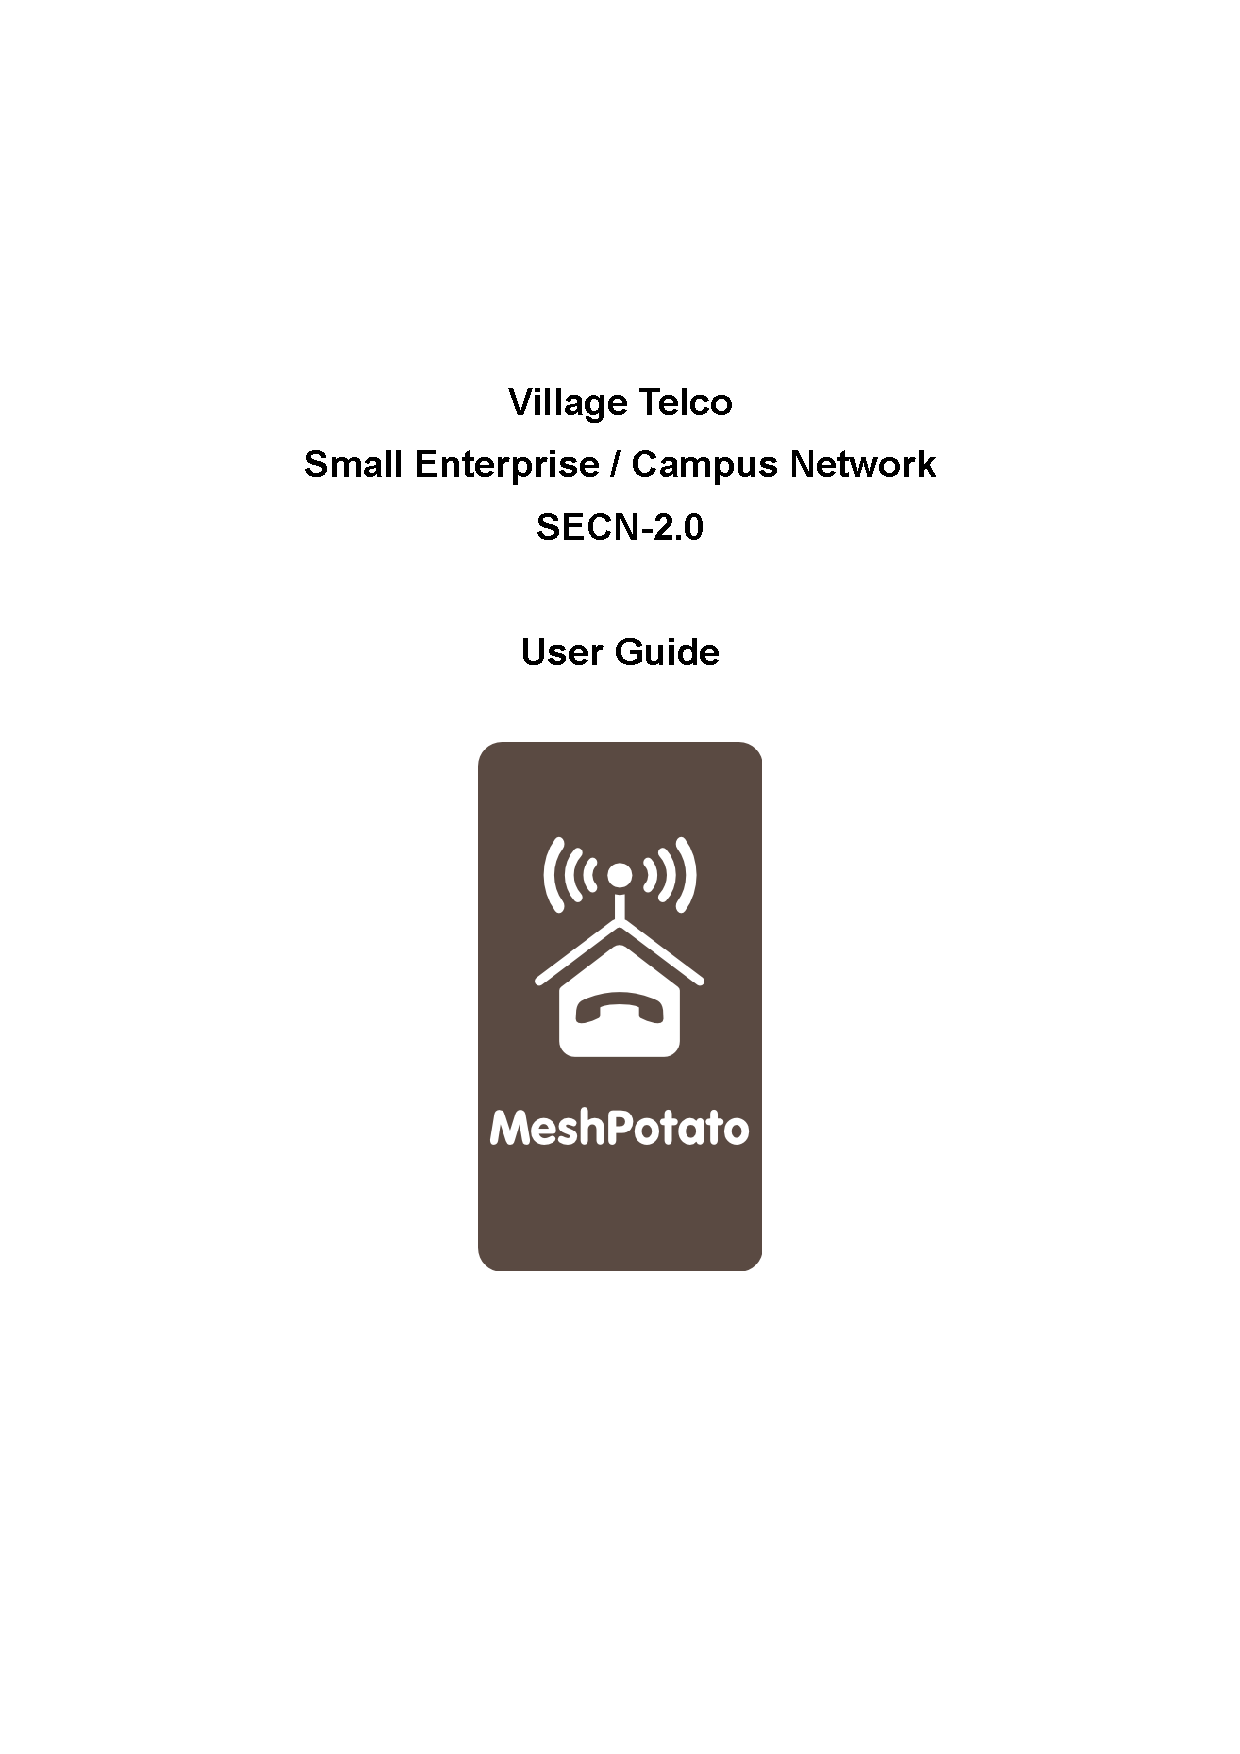
\includepdf[pages={1-46}]{SECN2.pdf}


\end{document} 
